\documentclass[11.5pt]{article}
\usepackage[table]{xcolor}
\definecolor{lightgray}{gray}{0.9}
\usepackage{multirow} 
\usepackage{lscape}
\usepackage{filecontents}
\usepackage[left=2.5cm,top=2.5cm,right=2.5cm,bottom=2.5cm]{geometry}
\usepackage{amsmath}
\usepackage{array}
\usepackage{caption}
\usepackage{longtable}
\usepackage{placeins}
\usepackage{graphicx}
\usepackage{subcaption}
\usepackage{setspace}
\usepackage{animate}
%\usepackage[active,tightpage]{preview}
\usepackage{natbib}
\bibpunct{(}{)}{,}{a}{}{;} 
\usepackage{url}
\usepackage{nth}
\usepackage{authblk}
\usepackage{listings}
% for the d in integrals
\newcommand{\dd}{\; \mathrm{d}}
\newcommand{\tc}{\quad\quad\text{,}}
\newcommand{\tp}{\quad\quad\text{.}}
\bibliographystyle{apalike}

\title{Avoidable causes of death drive adulthood survival's stagnation and reversal in Mexican states, 1990-2015}

%\author[1]{Nancy Plascencia\thanks{nancy.plascemcia@agricomer.com}}
\author[1]{Jos\'e Manuel Aburto}
%\author[3]{Ainhoa Alustiza}
\author[2]{Tim Riffe}
\affil[1]{European Doctoral School of Demography}
\affil[1,2]{Max Planck Institute for Demographic Research}


\begin{document}

\maketitle

\begin{abstract}
We analyze trends in mortality for three large age groups from 1990 to 2010 for all 32 Mexican states, and compare these with a low mortality benchmark. We assess the impact of avoidable mortality on survival at the state level by sex. We apply demographic measures and use standard decomposition techniques to disentangle the effects of selected causes of death on trends in state health inequality. We find improvements in survival for the population aged 0 to 14, as they continuously approached the low mortality benchmark. However, the adult population aged 15 to 39 shows deterioration among males after 2006 in almost every state. Females on the whole converged toward the low mortality benchmark in the same age group. Adults aged 40 to 74 show an unexpected decrease in the low mortality benchmark, indicating universal deterioration in temporary life expectancy for this age group, albeit with wide variation between states. These findings support the case for reforms that treat all causes of death as public health priorities, and that target regional disparities in health.

\end{abstract}

\section*{Key messages}
\begin{itemize}
\item Improving survival among sub-populations is a goal of every developing country. Achieving such goal in the adult population in Mexico is proving to be a challenging since the 1990s.
\item Geographic variation in the rise in homicide mortality and the increase of conditions amenable to medical services and policy/behavior actions are driving survival stagnation in adults.
\item Young-age mortality has steadily improved, mainly due to progress made in causes amenable to public health interventions.
\item Mexican states could benefit by two additional years of life if  cirrhosis, homicides, diabetes and isquemic heart diseases mortality were to achieve the low mortality benchmark 
\end{itemize}

\begin{spacing}{1.5}
\section*{Introduction (max 6000 words)}
The \nth{20} century was marked by sizable improvements in mortality, living
conditions and health in most Latin American countries \citep{who2000}. 
In Mexico, these improvements have slowed down recently as a result of opposing
trends in particular causes of death. For instance, homicide and diabetes
increased during the first decade of the 2000's, even as infectious and
respiratory diseases continued to fall over the same period. While life
expectancy at birth increased by 4.3 years for males (from 67.6 to 71.9) and 3.4
for females (from 73.8 to 77.2) between 1990 and 2000 \citep{SOMEDE},
between 2000 and 2010, life expectancy at birth entered into a period of
stagnation for males and slowed progress for females \citep{canudas2014}. 


This
period coincides with the implementation of different public health
interventions, such as the Universal Vaccination Program and Seguro
Popular, which aim to provide primary and secondary
health care to the uninsured population and allocate funds to cover catastrophic
health expenditures \citep{knaul2005}. Further, the conditional cash transfer program PROSPERA ( known as Oportunidades and Progresa before 2014)
was introduced to supply incentives for families to reinvest in education, health, and nutrition in 1997 \citep{neufeld2012}. Some evidence
suggests that Mexico experienced substantial decreases in infant and child
mortality, along with improvements that contributed to the reduction of
mortality and in the prevalence of acute malnutrition between 1980 and 2000
because of these interventions \citep{sepulveda2006}. Similarly, by 2012 Seguro Popular had provided health insurance coverage to an additional 52 million
people in Mexico that previously did not have any access to public health care and, as a result, there has been a reduction in catastrophic health expenditures \citep{knaul2012}.

These results underscore broad progress in public health interventions, but they mask heterogeneity between Mexican states and the epidemiological patterns for different age groups. Therefore, it is necessary to assess the varied impacts that these interventions may have had on mortality in Mexican states. For instance, PROSPERA is focused on the poorest states, and Seguro Popular was introduced at different times in different states. In addition, Mexico faces a rapid aging process in which we can anticipate the interaction between infectious diseases and noncommunicable conditions \citep{Bygbjerg1499}, such as diabetes, on the adult population.\footnote{The percentage of the population aged 60 or older will go from 10\% in 2015 to 15\% in 2030 according to projections made by \citet{CONAPO}} Identifying specific opportunities to improve and put forward solutions to reduce the gap of  the unequal impact of public health interventions on health is a necessary step to promote equitable increases in survival among the Mexican population.% the high degree of social and health inequalities present in the country \citep{Frenk2006} 
% In addition,  given the improvements in health care coverage, the strong role %of institutions, and ongoing public
 %health interventions, 
 
 One approach to assess the impact of health care and other interventions is by operationalizing the
 concept of Avoidable or Amenable Mortality (hereafter abbreviated AM)
 \citep{nolte&mckee2004, nolte&mckee2008,elo2014}. This categorization of mortality aims to measure the quality of health service systems by selecting certain
 causes of death that should not occur in the presence of effective and
 timely health care. Among industrialized countries, such as United States,
 Australia, France, Japan, a reduction in AM rates was
 observed over the part 20 years
 \citep{nolte&mckee2008}. Avoidable mortality rates fell, on average, by 17\%
 for males and 14\% for females in these countries. Despite mortality reductions from cancers and circulatory diseases for
 both sexes, heterogeneity between countries persists, with the United
 States showing the smallest reductions (around 5\%) for both sexes  \citep{nolte&mckee2008}. 
 
 In Mexico, the components of avoidable mortality had different trends since the
late 1990's. Between 2000 and 2004 AM decreased, particularly from
infectious diseases and nutrition-related conditions \citep{francomarina2006}, while it increased between 1998 and 2010 due to diabetes, circulatory diseases, perinatal and respiratory conditions
\citep{agudelo2014efecto}. Increases in the latter causes
of death were particularly concentrated in the poorest states of the country
\citep{davila2014mortalidad}. We aim to extend these studies
by a more focused segmentation of AM into health intervention-related AM and
behavior-related AM. Also, we extend analysis to all 32 states, by sex, and over
the full 26-year period from 1990 to 2015. Finally, we compare state mortality patterns
with an easy-to-understand low-mortality benchmark calculated for large age groups (e.g., 0-14, 15-39, 40-75). This low mortality
benchmarks is calculated on the basis of the lowest observed mortality within
ages and causes, selected from the full set of 32 Mexican states. This concept was first
proposed by \citet{whelpton1947} and later explored by  \citet{wunsch1975minimum} and
\citet{vallin2008minimum}. Deviations from the low-mortality benchmark indicate a strong potential for improvement. We apply demographic measures and
standard decomposition techniques to isolate the cause and age-specific deviations between states and the low mortality optimal lifetable for each year.

We hypothesize age-dependent variations in mortality outcomes.
In particular, we expect convergence between states and improvement in survival
for young people, since public health interventions are mainly focused in infant
mortality and child health. For instance, the vaccination program and the health
reform aim to fully cover children in the entire country, and recent
evidence suggests a decrease in mortality between ages 0 to 14 due to a decline
in infectious and respiratory diseases \citep{canudas2014}. On the contrary, we
expect little improvements in survival for the  young-adult population due to the unprecedented rise in homicide mortality, and on the older adults because of the increase in diabetes mortality along with endocrine/metabolic diseases in these ages in the country \citep{canudas2014}. Although every
state has the commitment to providing universal coverage and equitable access to
health care since the early 2000's, we anticipate heterogeneity between states
in mortality improvements due to state differences in epidemiological patterns and differences in how  health care programs have been delivered to the population
\citep{Frenk2006}.


\section*{Data \& Methods} 
Our analyses are based on publicly available anonymized datasets. We used deaths microdata available from official files produced by the
Mexican Statistical Office from 1990 to 2015 \citep{INEGI}. These data contain
information on causes of death by single age, sex, and state of residence at the
time of death. Population estimates from 1990 to 2015 came from the Mexican Society of Demography. These estimates adjust for age misstatement, undercounting, and interstate and international migration. Death counts and estimated of the population exposed to risk were used to calculate cause-age-specific death rates by sex and state from 1990 to 2015.
%Additionally, we estimate intercensal population counts by age, sex and state for the period 2011-2014 using the most recent inter-census survey that took place in 2010  \citep{INEGI}. Note: this is not possible the way we thought to do it, I did some estimations and had unsatisfactory results, some cases with crazy exposures, I think mainly because the results for 2015 are still not corrected for age miss-statement. Options: use CONAPO exposures, they are forecasted 5 years or wait to the new estimates.

\subsection*{Classification of Causes of Death}

To separate causes of death that are susceptible to medical intervention (such as
infectious and respiratory diseases) and those related to health behaviors and
intersectoral policies (such as homicides, lung cancer) we use the concept of
``Avoidable/Amenable Mortality'' (AM) \citep{nolte&mckee2004, nolte&mckee2008}. We group causes of death into ten categories based on \citet{elo2014}'s classification, recently complemented to the  Mexico's case \citep{Aburto2015}, as listed in Table~\ref{tab:causes}, with relative frequencies by sex for the period 2000-2015.

% latex table generated in R 3.2.2 by xtable 1.8-0 package
% Mon Feb  8 21:50:32 2016
% latex table generated in R 3.2.2 by xtable 1.8-0 package
% Mon Feb  8 21:52:20 2016
\begin{table}[ht]
\centering
\caption{Avoidable Mortality classification, 
             with crude percentages below age 75, years 1990-2010. Source: INEGI files.} 
\label{tab:causes}
\begin{tabular}{lllll}
  \hline
Category &\% & Males &  \% & Females \\ 
 && (1,000's) & & (1,000's)\\ 
  \hline
Causes amenable to medical service &                             28.5 \% &                              1,131 &                             40.2 \% &                              1,067 \\ 
                            Diabetes &                              9.1 \% &                                360 &                             14.8 \% &                                392 \\ 
             Ischemic heart diseases &                              7.9 \% &                                314 &                              6.7 \% &                                177 \\ 
                            HIV/AIDS &                              1.8 \% &                                 72 &                              0.5 \% &                                 14 \\ 
                         Lung cancer &                              1.6 \% &                                 63 &                              1.1 \% &                                 29 \\ 
                           Cirrhosis &                              5.3 \% &                                212 &                              1.1 \% &                                 29 \\ 
                            Homicide &                                6 \% &                                236 &                                1 \% &                                 28 \\ 
              Road traffic accidents &                              5.8 \% &                                231 &                              2.3 \% &                                 60 \\ 
                             Suicide &                              1.5 \% &                                 59 &                              0.5 \% &                                 12 \\ 
                        Other causes &                             32.5 \% &                              1,291 &                             31.9 \% &                                845 \\ 
   \hline
\end{tabular}
\end{table}

% latex table generated in R 3.1.2 by xtable 1.7-4 package
% Wed Sep 23 21:57:18 2015
%\begin{table}[ht]
%\centering
%\caption{Avoidable Mortality classification, with crude percentages below age 75.}
%\label{tab:causes}
%\begin{tabular}{>{\raggedright}m{3cm}rr}
%Group/Cause  & Males & Females \\ 
%  \hline
%Causes amenable to medical service & 28.50 & 40.24 \\ 
%  Diabetes & 9.07 & 14.77 \\ 
%  Ischemic heart diseases & 7.92 & 6.66 \\ 
%  HIV/AIDS & 1.80 & 0.51 \\ 
%  Lung cancer & 1.58 & 1.09 \\ 
%  Cirrhosis & 5.34 & 1.09 \\ 
%  Homicide & 5.95 & 1.05 \\ 
%  Road traffic accidents & 5.82 & 2.26 \\ 
%  Suicide & 1.48 & 0.46 \\ 
%  Other causes & 32.53 & 31.86 \\ 
%   \hline
%\end{tabular}
%\end{table}

We separate diabetes, ischemic heart diseases (IHD), HIV/AIDS, lung
cancer, and cirrhosis because these causes are susceptible to both health behavior
and medical service, and because the first two represent major causes of death
in Mexican adults \citep{canudas2014}. We also separate
homicide, road traffic accidents, and suicide because they have emerged as
leading causes of death among young people, and the first two had a sizeable
impact on life expectancy recently in Mexico \citep{canudas2014}. All causes of death were classified using the International Classification of Diseases, revision 9 for the period 1990-1997 and the tenth revision for 1998-2010 (see Appendix Table 1 for details on ICD codes for each cause). To avoid spurious results concerning the change in coding practices between the ninth and tenth revision, we performed a sensitivity analysis and did not find major changes in mortality trends by AM classification (See Appendix figure \ref{fig:ClassSens}). Although ill-defined causes represent a small percent of the total deaths (2\% in 1992 \citep{rivera2002epidemiological}), we decided to leave them in the residual category because if we spread them proportionally,  among the other causes of death could over estimate our results.

We truncated analysis at age 75 because classification of causes of deaths and age reporting are considered to be innacurate in death registration at older ages \citep{tobias2001} and most changes in life expectancy are likely due to changes in mortality patterns below the age of 75 \citep{Aburto2015}. 

\subsection*{Age Groups}

We break life expectancy into three large age groups to capture mortality differences along the lifespan based on previous research. The first group refers to people aged 0-14. This group is likely to represent improvements in causes amenable to medical service (e.g. infectious diseases and conditions of perinatal period) \citep{canudas2014}. The second group, aged 15-39, is used to capture the effect of homicide mortality and external causes, which have an important impact on life expectancy in these ages \citep{Aburto2015}. Finally, the third group is for older adults aged 40-74. 
We focus on older adults because they are susceptible to external causes of death and likely to experience premature death due to noncommunicable conditions \citep{canudas2014}.

\subsection*{Demographic Methods}
We smooth cause-specific death rates over age and time for each
state and sex separately using the 2-d p-spline method proposed by
\citet{GC2012} to avoid random variations between ages. Smoothed death rates are
then constrained to sum to the unsmoothed all-cause death rates. We then calculate period life tables up to
age 74 for males and females from 1990 to 2010 following the HMD Methods
Protocol \citep{HMDMP}. We calculate the average years lived in each age group (temporary life expectancy) \citep{arriaga1984} (See Appendix for a technical overview) and estimate cause-specific contributions to the difference between
state-specific temporary life expectancy and  the low mortality benchmark. We use
 standard decomposition methods \citep{horiuchi2008}.

\subsection*{Low mortality benchmark}
Our low-mortality benchmark is calculated in the basis of the lowest observed mortality rates by age, cause of death, from among all states for a given sex and year.


%The low mortality rates $\mu(x)^\star$, are calculated as the sum of $C$ cause-specific minimum %mortality rates at age $x$, under the assumption that causes of deatg are independent of one another:
%\begin{equation}
%\label{eq:mxmin}
%\mu(x)^{\star} = \sum_c=1^C min(\mu(x,c,s))
%\end{equation}
%where $x$ is age, $c$ is the given cause of death, and $s$ indexes the set of 32 states from which %the minimum is selected. 

The resulting minimum mortality rate schedule has a unique age profile, and it determines our benchmark temporary life expectancy, $e(0)^\star$. The minimum mortality schedule can be treated as the best presently achievable mortality assuming perfect diffusion of the best available practices and technologies within a given set of populations \citep{vallin2008minimum}. It is an imaginary quantity because no particular population is expected to achieve this mortality pattern. However, this value is a practical reference because it is based neither on a projection of improvements into the future nor on an arbitrary and likely dissimilar population. We refer to the state with the highest life expectancy in a given year as the vanguard state.


\subsection*{Limitations}
Mortality data from Mexico are
likely to present inaccuracies in cause-of-death classification due to
comorbidities, particularly at older ages \citep{tobias2001}. To mitigate this,
we focus on ages below 75, grouping causes of death using ICD codes.
Our estimates regarding homicide mortality are likely to be
underestimated due to inaccurate practices regarding counting, reporting,
and due to the large number of ``missing'' individuals in Mexico \citep{HRW2011}.

Avoidable mortality should be understood as an indicator of potential
weaknesses with respect to health care and some public health policies and not
as a definitive assessment \citep{nolte&mckee2008}. The amount of deaths that should be considered avoidable within the avoidable classification is not clear \citep{beltran2011avoidable}. For instance, some authors consider only 50 percent of heart diseases as avoidable \citep{nolte2012amenable}

We do not have information to precisely
measure percentages of avoidable mortality within cause groups in Mexico. Nonetheless, the
difference between a given mortality schedule and the best mortality schedule of
the same year can be conceived of as a minimal definition of avoidable
mortality. The benchmark mortality schedule sets a lower bound to how much mortality could have been avoided. Certainly, even the best mortality schedule will contain elements of mortality that
most would consider avoidable. To the extent that the components of the benchmark schedule were indeed
attained somewhere in the population universe, one can view any excess mortality
with respect to the benchmark schedule as avoidable. Little progress has been made in advancing the concept of avoidable mortality \citep{holland2003}. We believe this perspective improves on the original concept by giving a directly measurable standard against which to estimate avoidable deaths.


\section*{Results}
\subsection*{Trends in the low mortality benchmark and temporary life expectancy}
Figure 1 presents the state-specific trends in temporary life expectancy for young, young-adult and older-adult populations (black lines). The red lines represent the record holder state in a given year, while the blue line represents the low mortality benchmark. Panel a) shows the trend of convergence and improvements among the young population. Since the 1990's all the states have shown improvements towards the low mortality benchmark, approaching near-complete survival between ages 0 and 14. However, both males and females have lagged behind in states such as Puebla, Tlaxcala and M\'exico.

Opposing this trend, temporary life expectancy between 15 and 39 years shows a common shift after 2005 in almost every state in Mexico  (panel b)). Chihuahua and Sinaloa, in the Northern region, experienced the largest downwards trends after 2005. Over the full period Oaxaca, Baja California, and Chihuahua  show the largest departures from the low mortality benchmark. Results for females show stagnation close to the maximum attainable survival. However,  as in males' results, Chihuahua exhibit reductions in survival after 2005.

Temporary life expectancy for adults between 40 and 75 years shows stagnation and deterioration during the entire period (panel c)). Even the low mortality benchmark exhibits a gradual downward trend, pointing to increases in adult mortality in every state. From a potential maximum of 35 years, 
all the states are living on average less than 30 years for males and 32 for females. Importantly,  Baja California, Chihuahua and Sonora could potentially live more than two additional years if the low mortality benchmark were achieved for males. Similar to the young-adult males, some states experienced a  clear downward trend after 2005. Results for females show stagnation in this age-group. 

These results allow us to identify three different patterns between the age groups and states. Mortality in ages 0-14 has been decreasing, approaching almost complete survival. Adults aged 15-39, particularly males, present a clear reversal in temporary life expectancy after 2005. Males and females aged 40-74 showed stagnation and deterioration since the 1990's. This has led to a 2-year gap for males and 1-year gap for females with benchmark survival, which itself falls short of the full 25 years by almost 3 years for males and 2.2 for females. To fully understand the underlying causes of death driving these stories, we decompose the gap between state-specific temporary life expectancy and the low mortality benchmark within each age-group.


\begin{figure}
\label{Fig_temporary_le}
\centering
\caption{Temporary life expectancy for states (black line), record life
expectancy (red) and low mortality benchmark by sex, 1990-2010.}
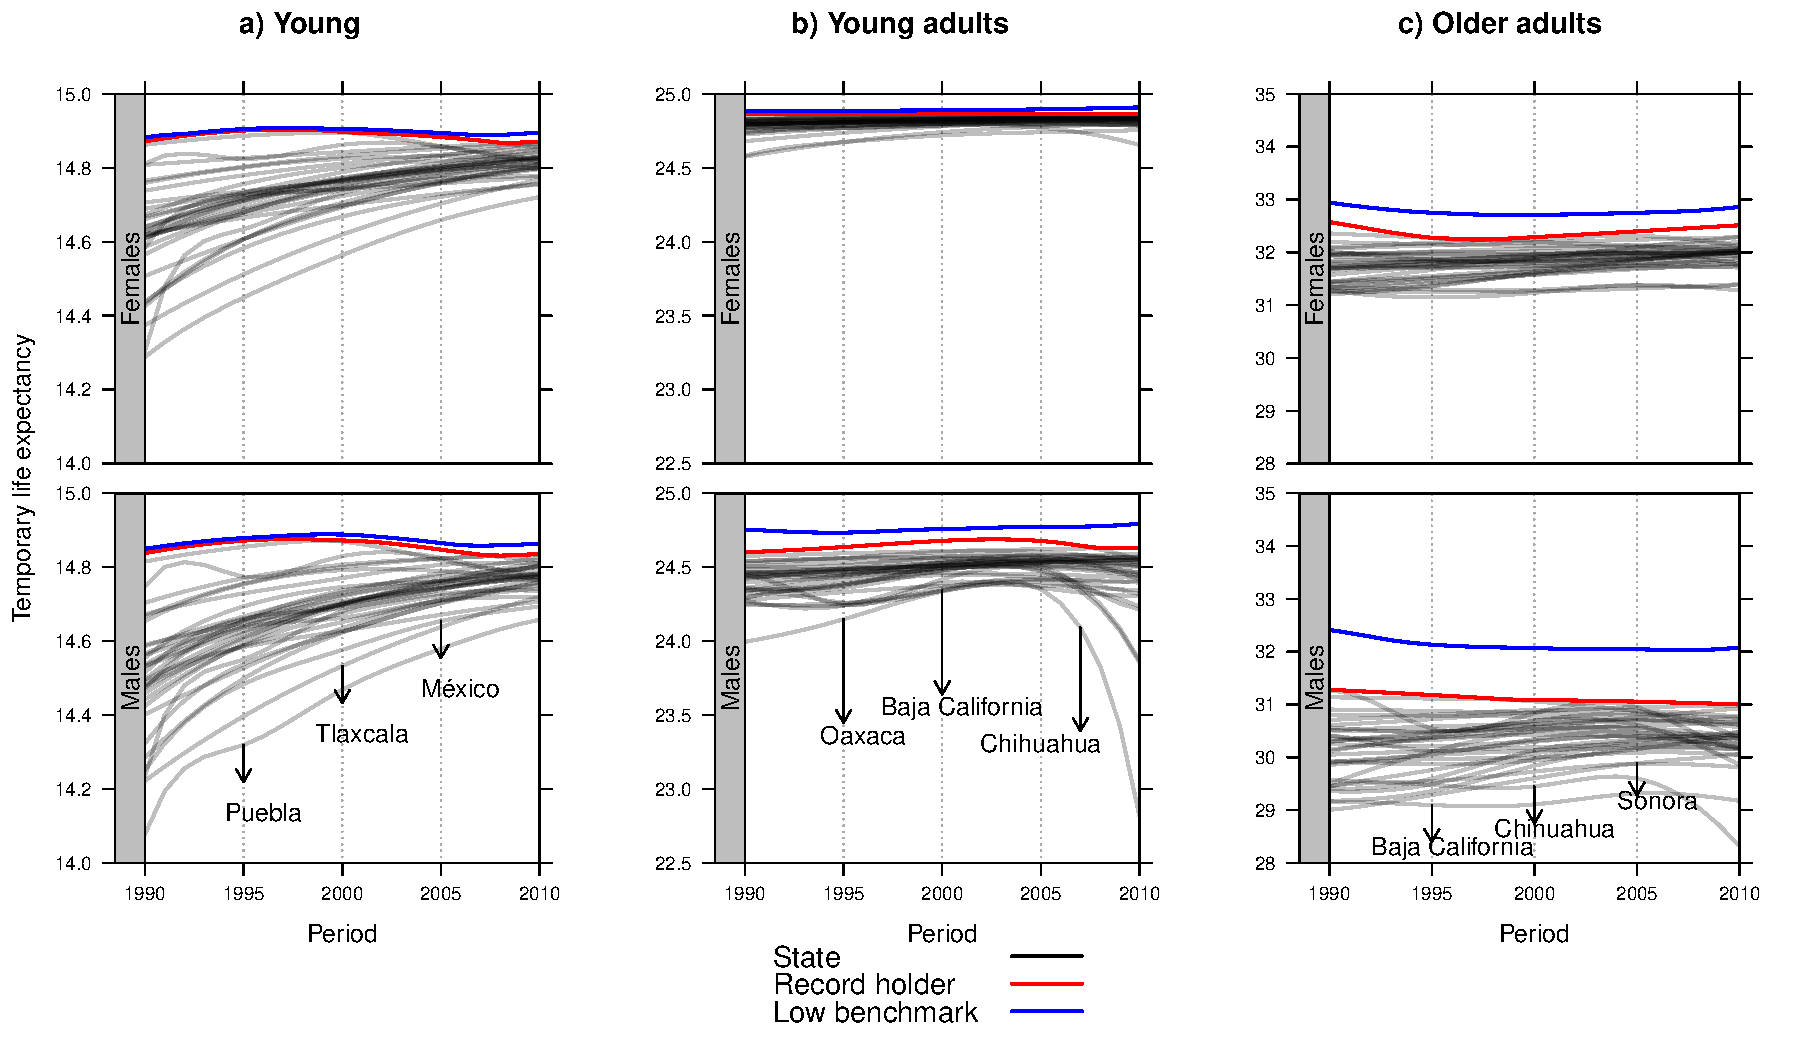
\includegraphics[scale=.5]{Figures/Temp_fig.pdf}

Note: Y-axis are not in the same scale in order to capture major trends over the period. Source: calculations based on INEGI and SOMEDE files. 
\end{figure}

%\FloatBarrier
%\subsection*{State trends in departures from best practices temp e(0)}
%Small multiples maps (time series of maps)


\subsection*{Causes of death}

Of the age groups studied, adults aged 35-74 show the largest deviations from the low mortality benchmark. Figures  \ref{fig:e40_74_females} and \ref{fig:e40_74_males} show cause-specific contributions to the gap between observed temporary life expectancy and the low mortality benchmark by state and region for females and males, respectively. Light-yellow colors indicate no contributions to the gap, which means that are very close to the low mortality benchmark within each category. Darker red hues indicate larger contributions to the gap. If a particular state is improving during the period, it shows a transition from red to light-yellow. 

As shown in figure \ref{fig:e40_74_females}, medically amenable causes of death still contribute to the gap between survival and the low mortality benchmark. However, improvements in this category throughout the period 1990-2010 helped reduce deviations in almost every state. Chihuahua, Coahuila and Baja California, in the Northern region, and Chiapas in the South exhibit the largest deviations from the low mortality benchmark as mortality due to these causes stagnated in both females and males. Opposing this, the increase of diabetes mortality among females has contributed to widening the gap between temporary life expectancy and the low mortality benchmark. Some states, like Tabasco in the South and Coahuila in the North, show a clear deterioration on the survival in the 2000's due to this cause of death. Isquemic heart diseases (IHD) is the the third most important cause of death contributing to differences with the mortality benchmark among regions. The impact of IHD on the survival of the females aged 35-74 is concentrated in the Northern region. Mortality related to cirrhosis contributes significantly to the difference with the benchmark mortality in the Central and Southern regions in female survival. Its contribution is such that in states such as Tlaxcala, Quer\'etaro, M\'exico and Hidalgo in the central area, this cause of death accounts with more than half a year of the difference with the benchmark. The rest of AM-categories do not contribute significantly to the gap between female survival and the low mortality benchmark, which means that they are very close to the latter.

\begin{figure}[h]
\centering
\caption{Cause-specific contributions to state differences from low mortality benchmark for older female adults, 1990-2010. States grouped into three regions.)}
\label{fig:e40_74_females}
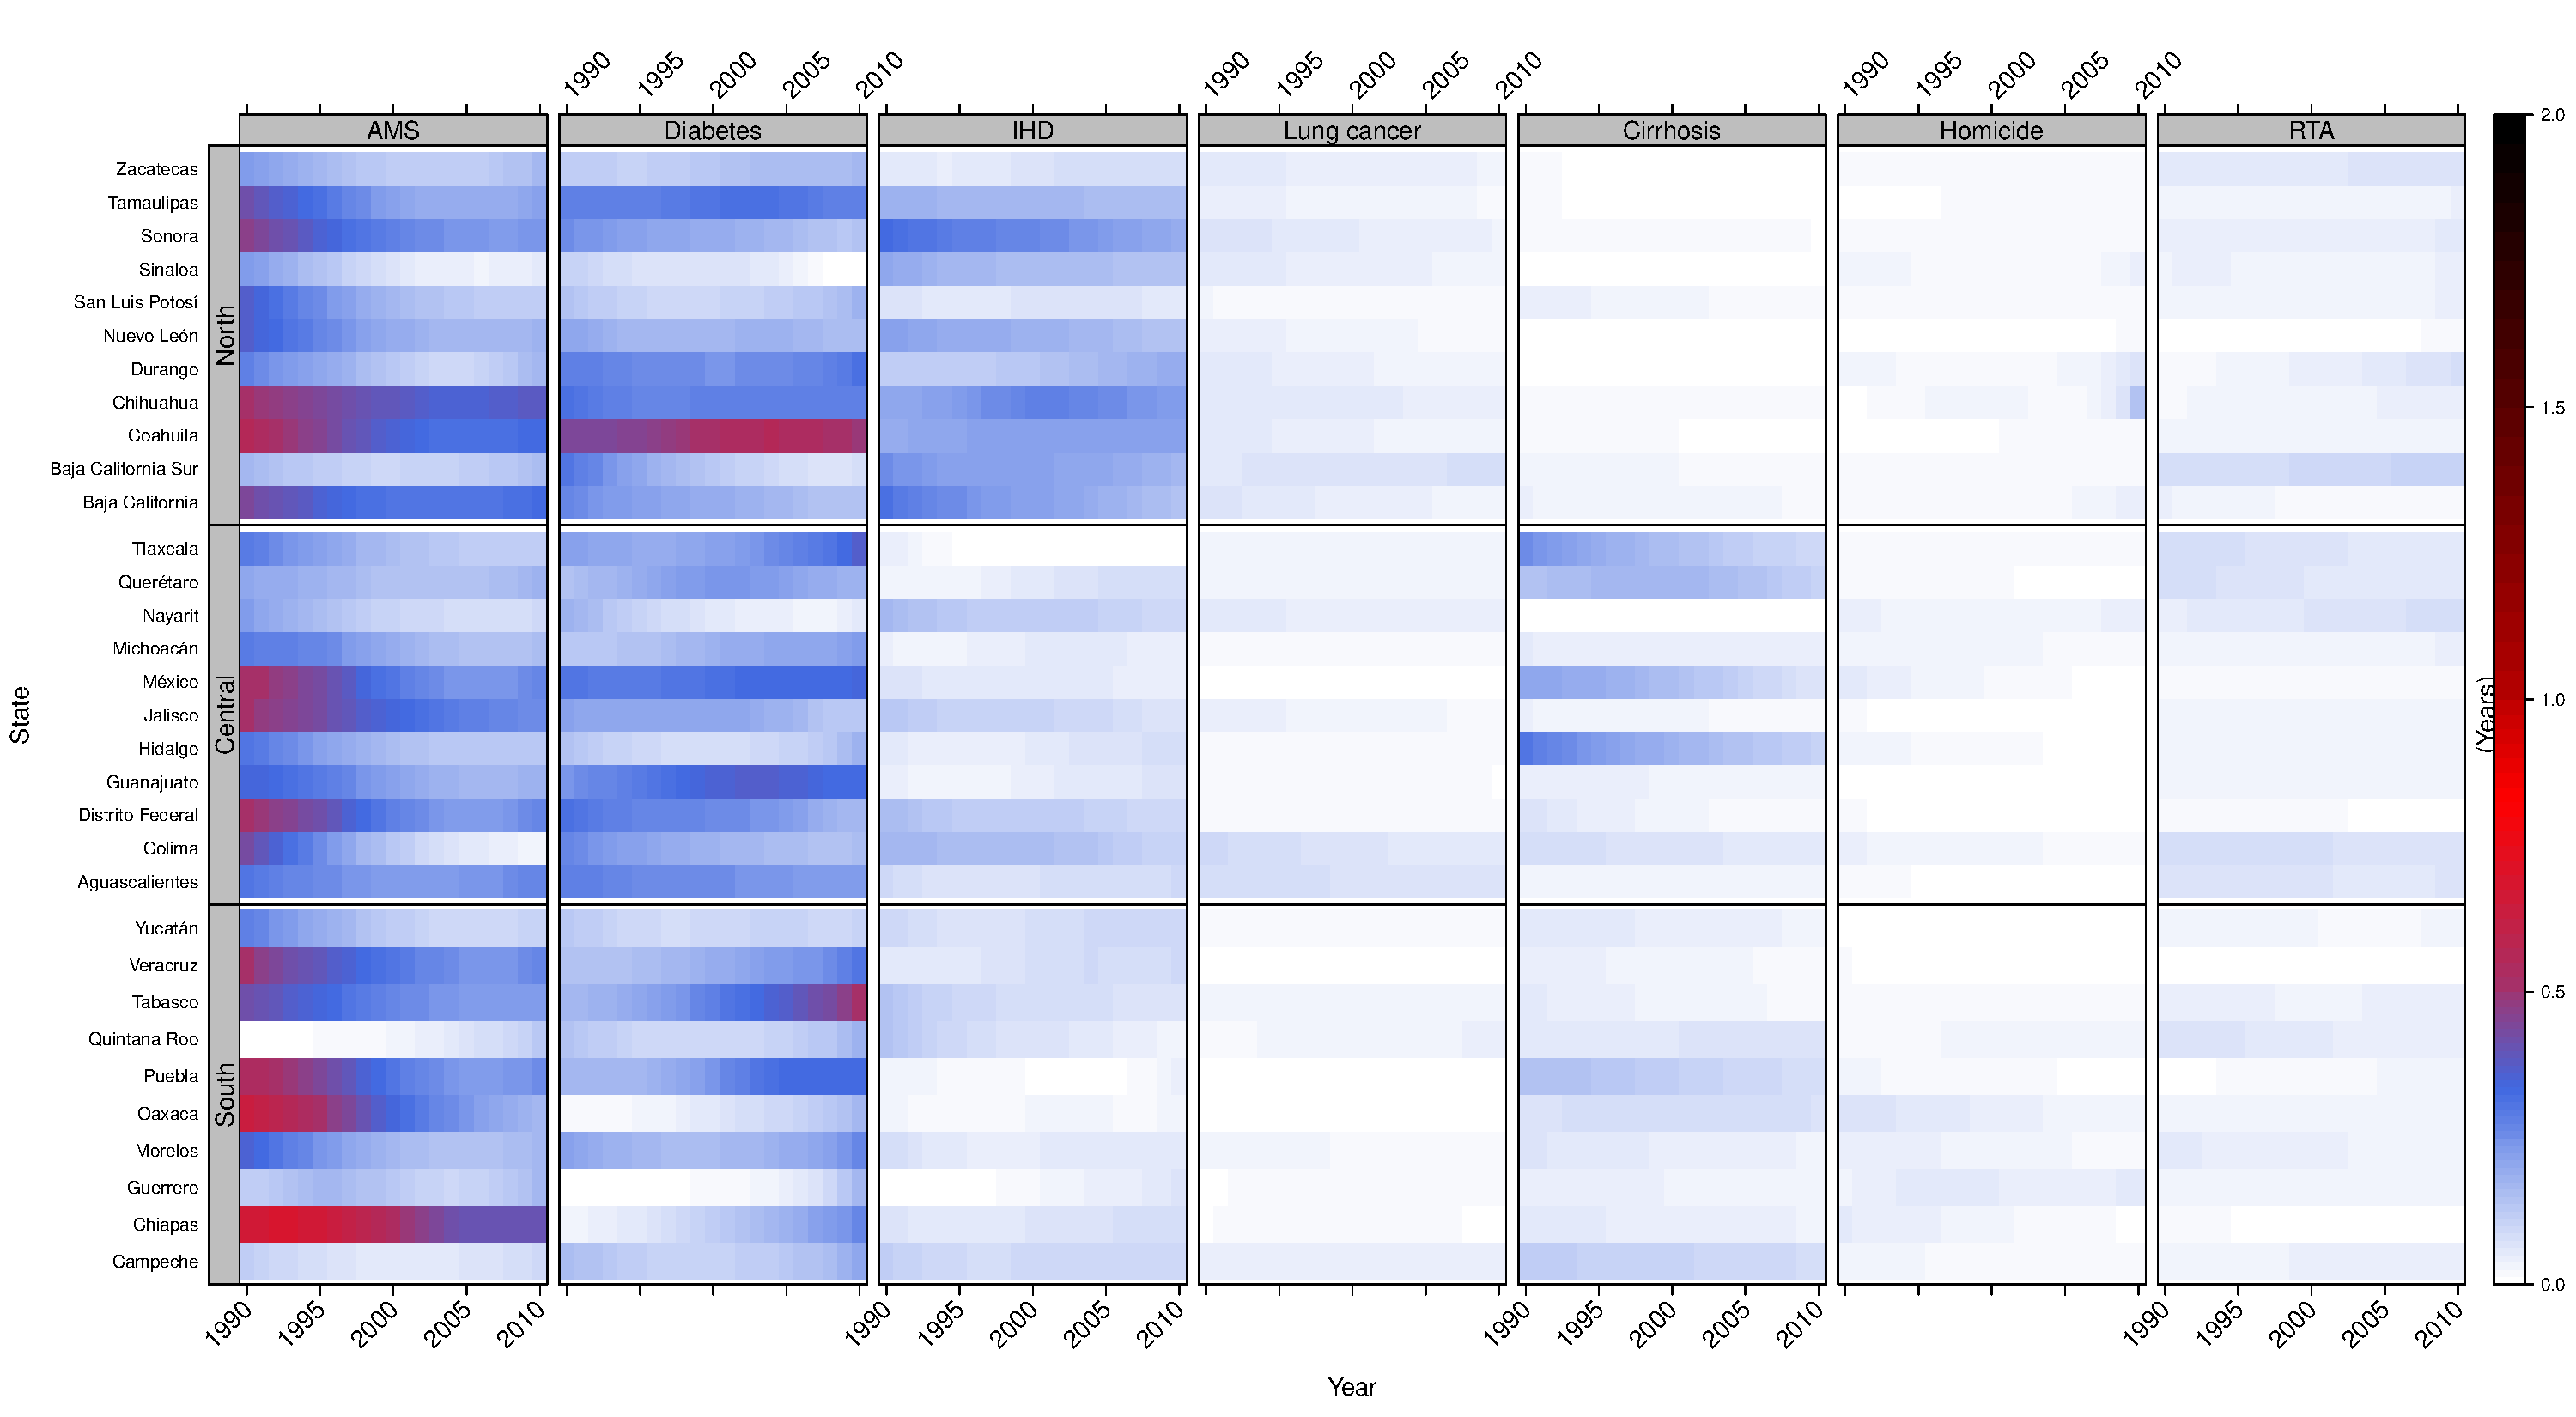
\includegraphics[scale=.33]{Figures/Adult_Female_heatmap.pdf}
Note: AMS is ``amenable to medical service'', IHD is ``isquemic heart diseases'', and RTA is ``road traffic accidents''. Source: calculations based on INEGI and SOMEDE files. \end{figure}

Causes amenable to medical service follow a similar pattern for males (figure  \ref{fig:e40_74_males}). However, diabetes, IHD and cirrhosis still contribute significantly to the difference between the observed mortality and the low mortality benchmark. The increase in diabetes has led to decreasing survival among male adults. For instance,  Tamaulipas, Coahuila (Northern area); Tlaxcala, M\'exico state, Guanajuato and the Federal District in the central region; along with Veracruz, Tabasco and Puebla in the South, show clear deterioration during the study period, while other states experienced improvements that led to reducing the gap towards the low mortality benchmark due to diabetes (such as Sinaloa in the North, Nayarit in the central region, and Yucat\'an in the South). As in females, IHD exhibit a very different pattern between regions. Nearly every state in the North could gain more than one year of life if IHD mortality were reduced to the low mortality benchmark. On the contrary, cirrhosis affects male survival mainly in the Central and Southern regions. Quer\'etaro, Michoac\'an, Jalisco, Puebla and Oaxaca show the largest deviations from the low mortality benchmark due to cirrhosis mortality. Finally, homicide mortality also affects older-adult survival in particular states, as the gaps between the low mortality benchmark and the observed life expectancy are wider after 2005. Similar to young adults patterns, Sinaloa, Durango, Chihuahua and Guerrero could potentially increase the survival in one year if homicide mortality converges to the low mortality benchmark. Nevertheless,  Michoac\'an and Oaxaca show gradual improvements over the last 20 years. Road traffic accidents (RTA) and the rest of AM-categories do not contribute notably to the gap between the observed survival and the low mortality benchmark. 




\begin{figure}[h]
\centering
\caption{Cause-specific contributions to state differences from low mortality benchmark for older male adults, 1990-2010.}
\label{fig:e40_74_males}
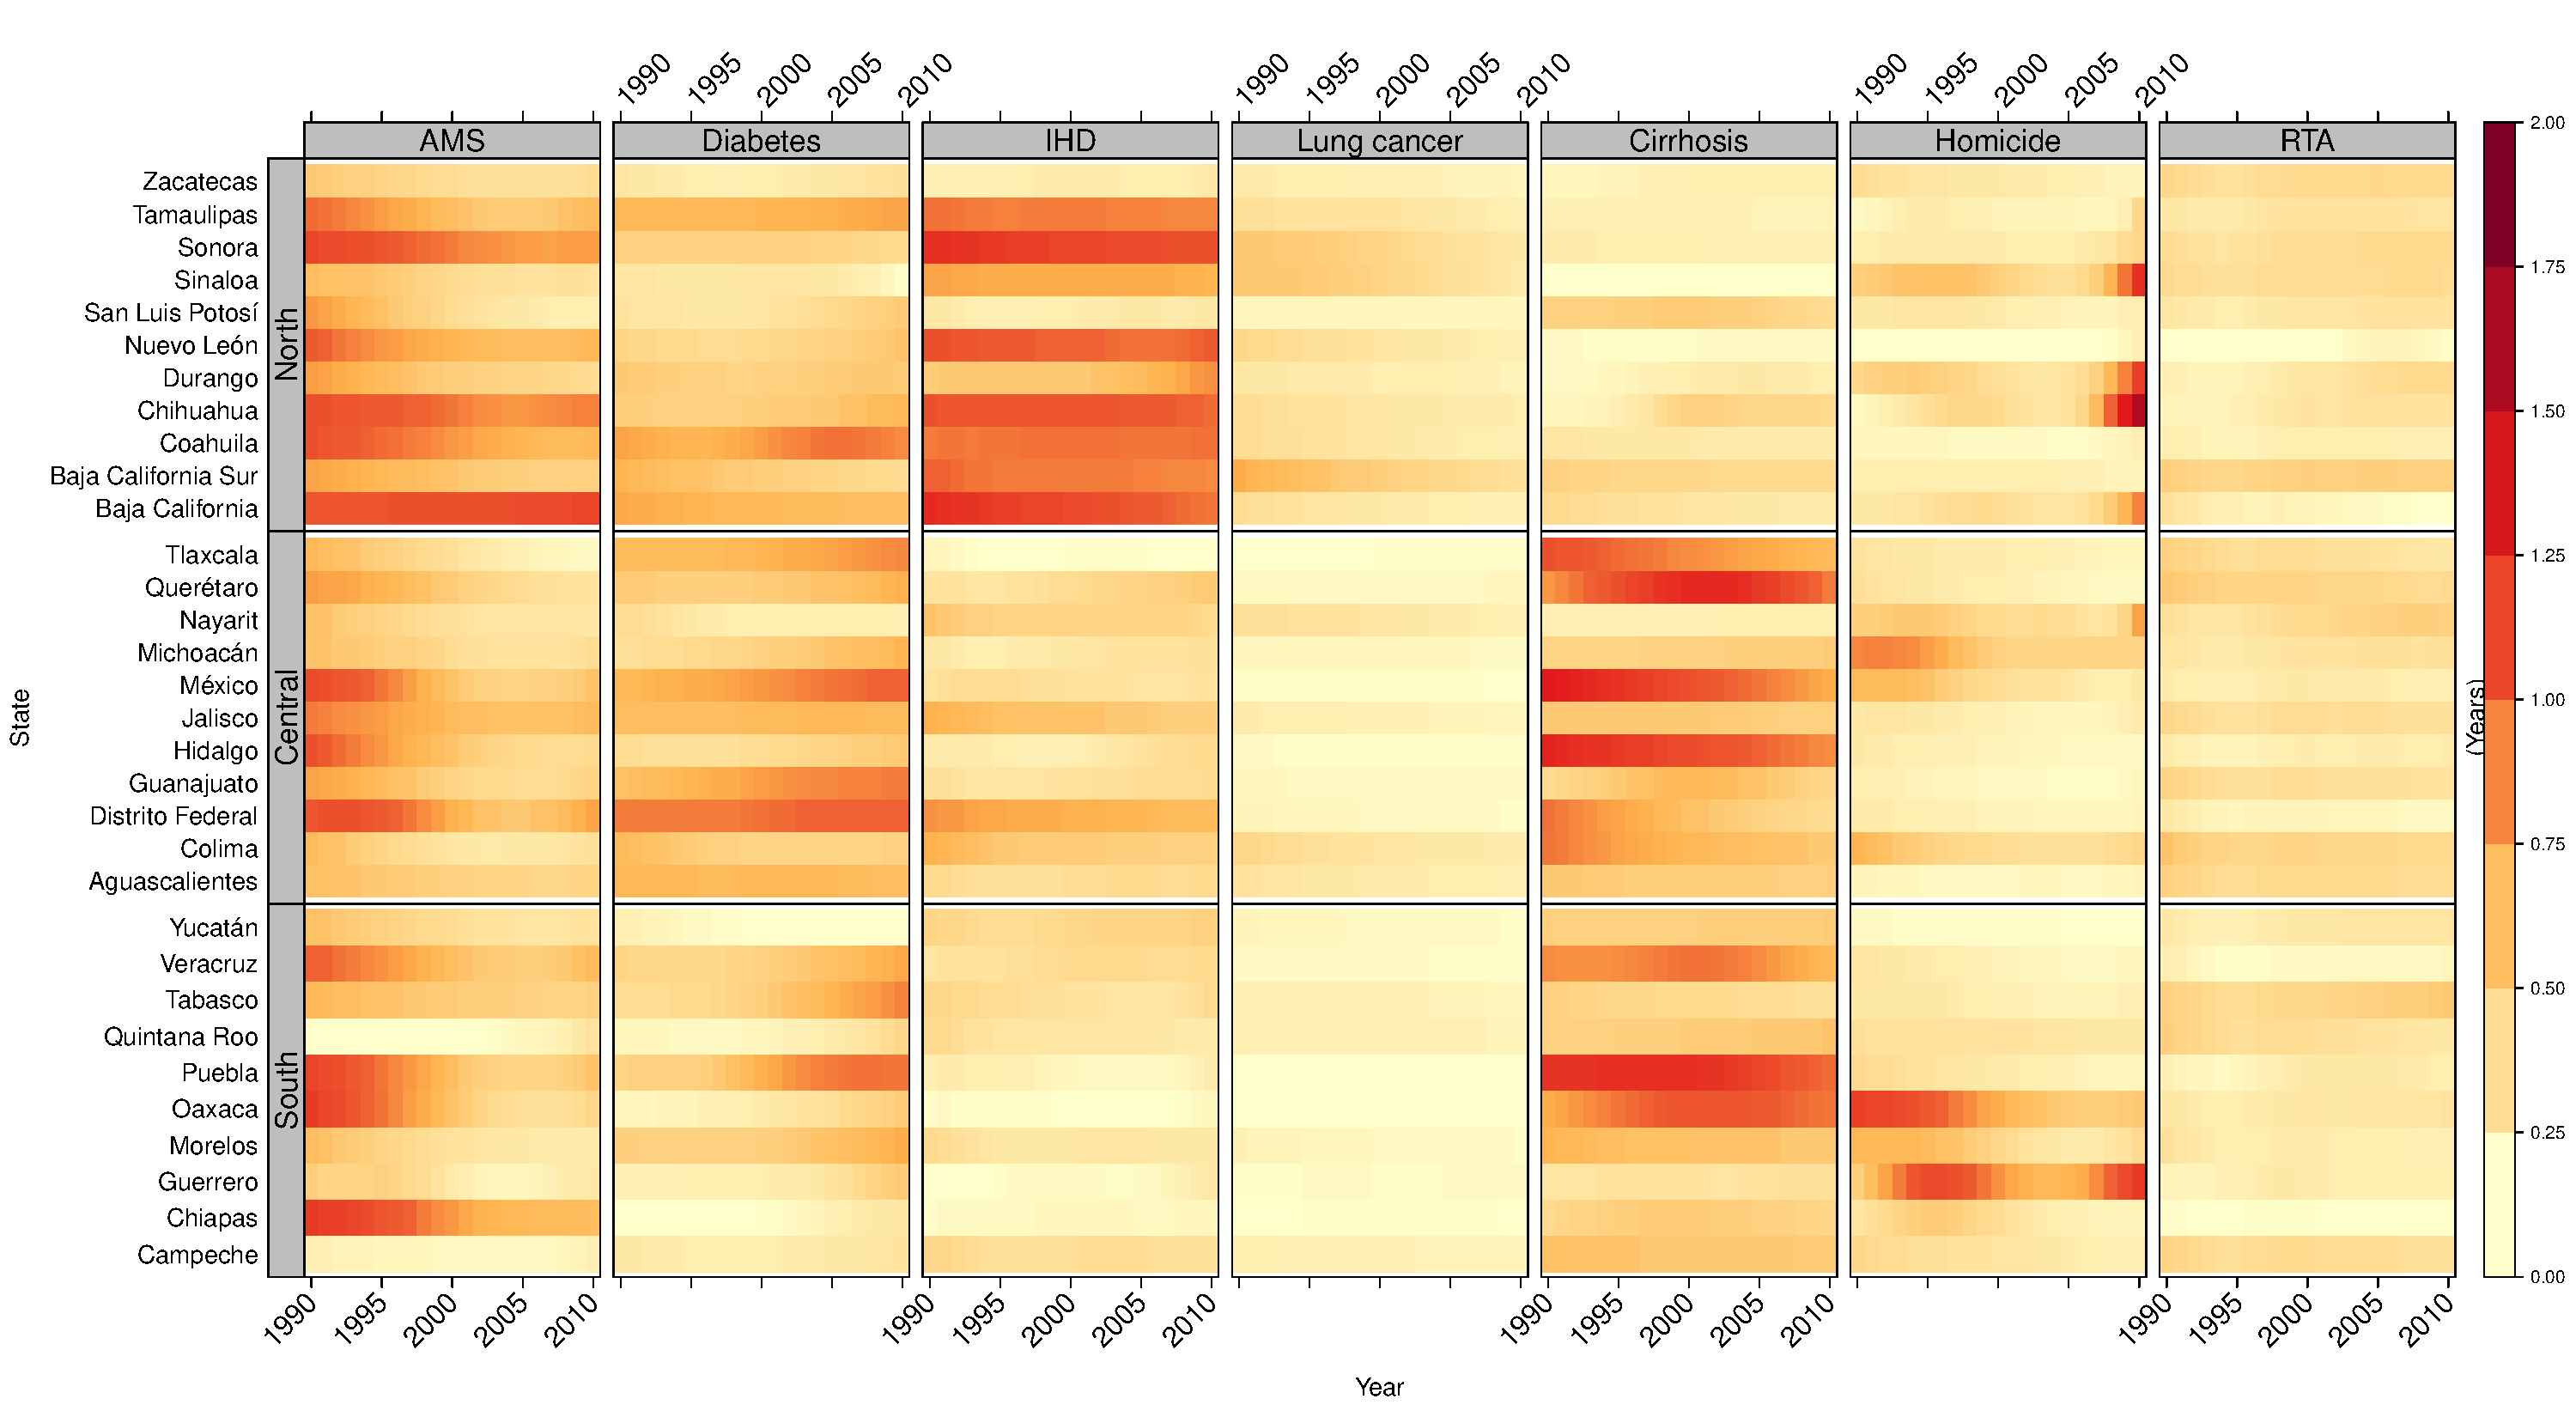
\includegraphics[scale=.33]{Figures/Adult_Male_heatmap.pdf}
Note: AMS, is the acronym for amenable to medical service, IHD for isquemic heart diseases and RTA stands for road traffic accidents. Source: own calculations based on INEGI and SOMEDE files. 
\end{figure}


Males and females in all 32 states increased survival between 0 and 14 due to reductions in causes amenable to medical service (see Appendix's figures  \ref{fig:e0_14_males} and \ref{fig:e15_39_males}). The convergence towards the low mortality benchmark was more intense in states in the Central and Southern region for males. For instance, Tlaxcala, Mexico, Puebla and Chiapas reduced the gap between the benchmark and the observed survival, gaining almost an entire additional year of life. 

Among the adult population aged 15-39, deviations from the low mortality benchmark observed in males after 2005 were mainly driven by homicide mortality (see Appendix's figure \ref{fig:e15_39_males}). The unexpected increase of homicide led to widening the gap between the benchmark and the observed survival in almost every state. In the Northern region, the gap went from around a quarter of year in 2002 to more than one year by 2010 in Sinaloa (pacific coast), Durango and Chihuahua (state bordering Texas in the U.S.). Nayarit, Michoac\'an, in the central region, and Guerrero in the South were the states that showed the largest deviations due to homicide mortality following trend otherwise observed only in the North. Road traffic accidents contributed to the gap between the benchmark and the observed temporary life expectancy but with a minor effect. In females, the gap due to homicide mortality after 2005 is only large in the state of Chihuahua (see Appendix figure \ref{fig:e15_39_females}). The impact of the remaining  AM categories in ages 0-14 and 15-39 is negligible. 



%\subsection*{Age and cause contributions to state differences from the best
%practices trend.}
%This section will be completed at a later date. Preliminary results are shown.
%\begin{figure}[h!]
%\caption{Cause-specific contributions to the difference between observed and BP. (preliminar figure)}
%\centering
%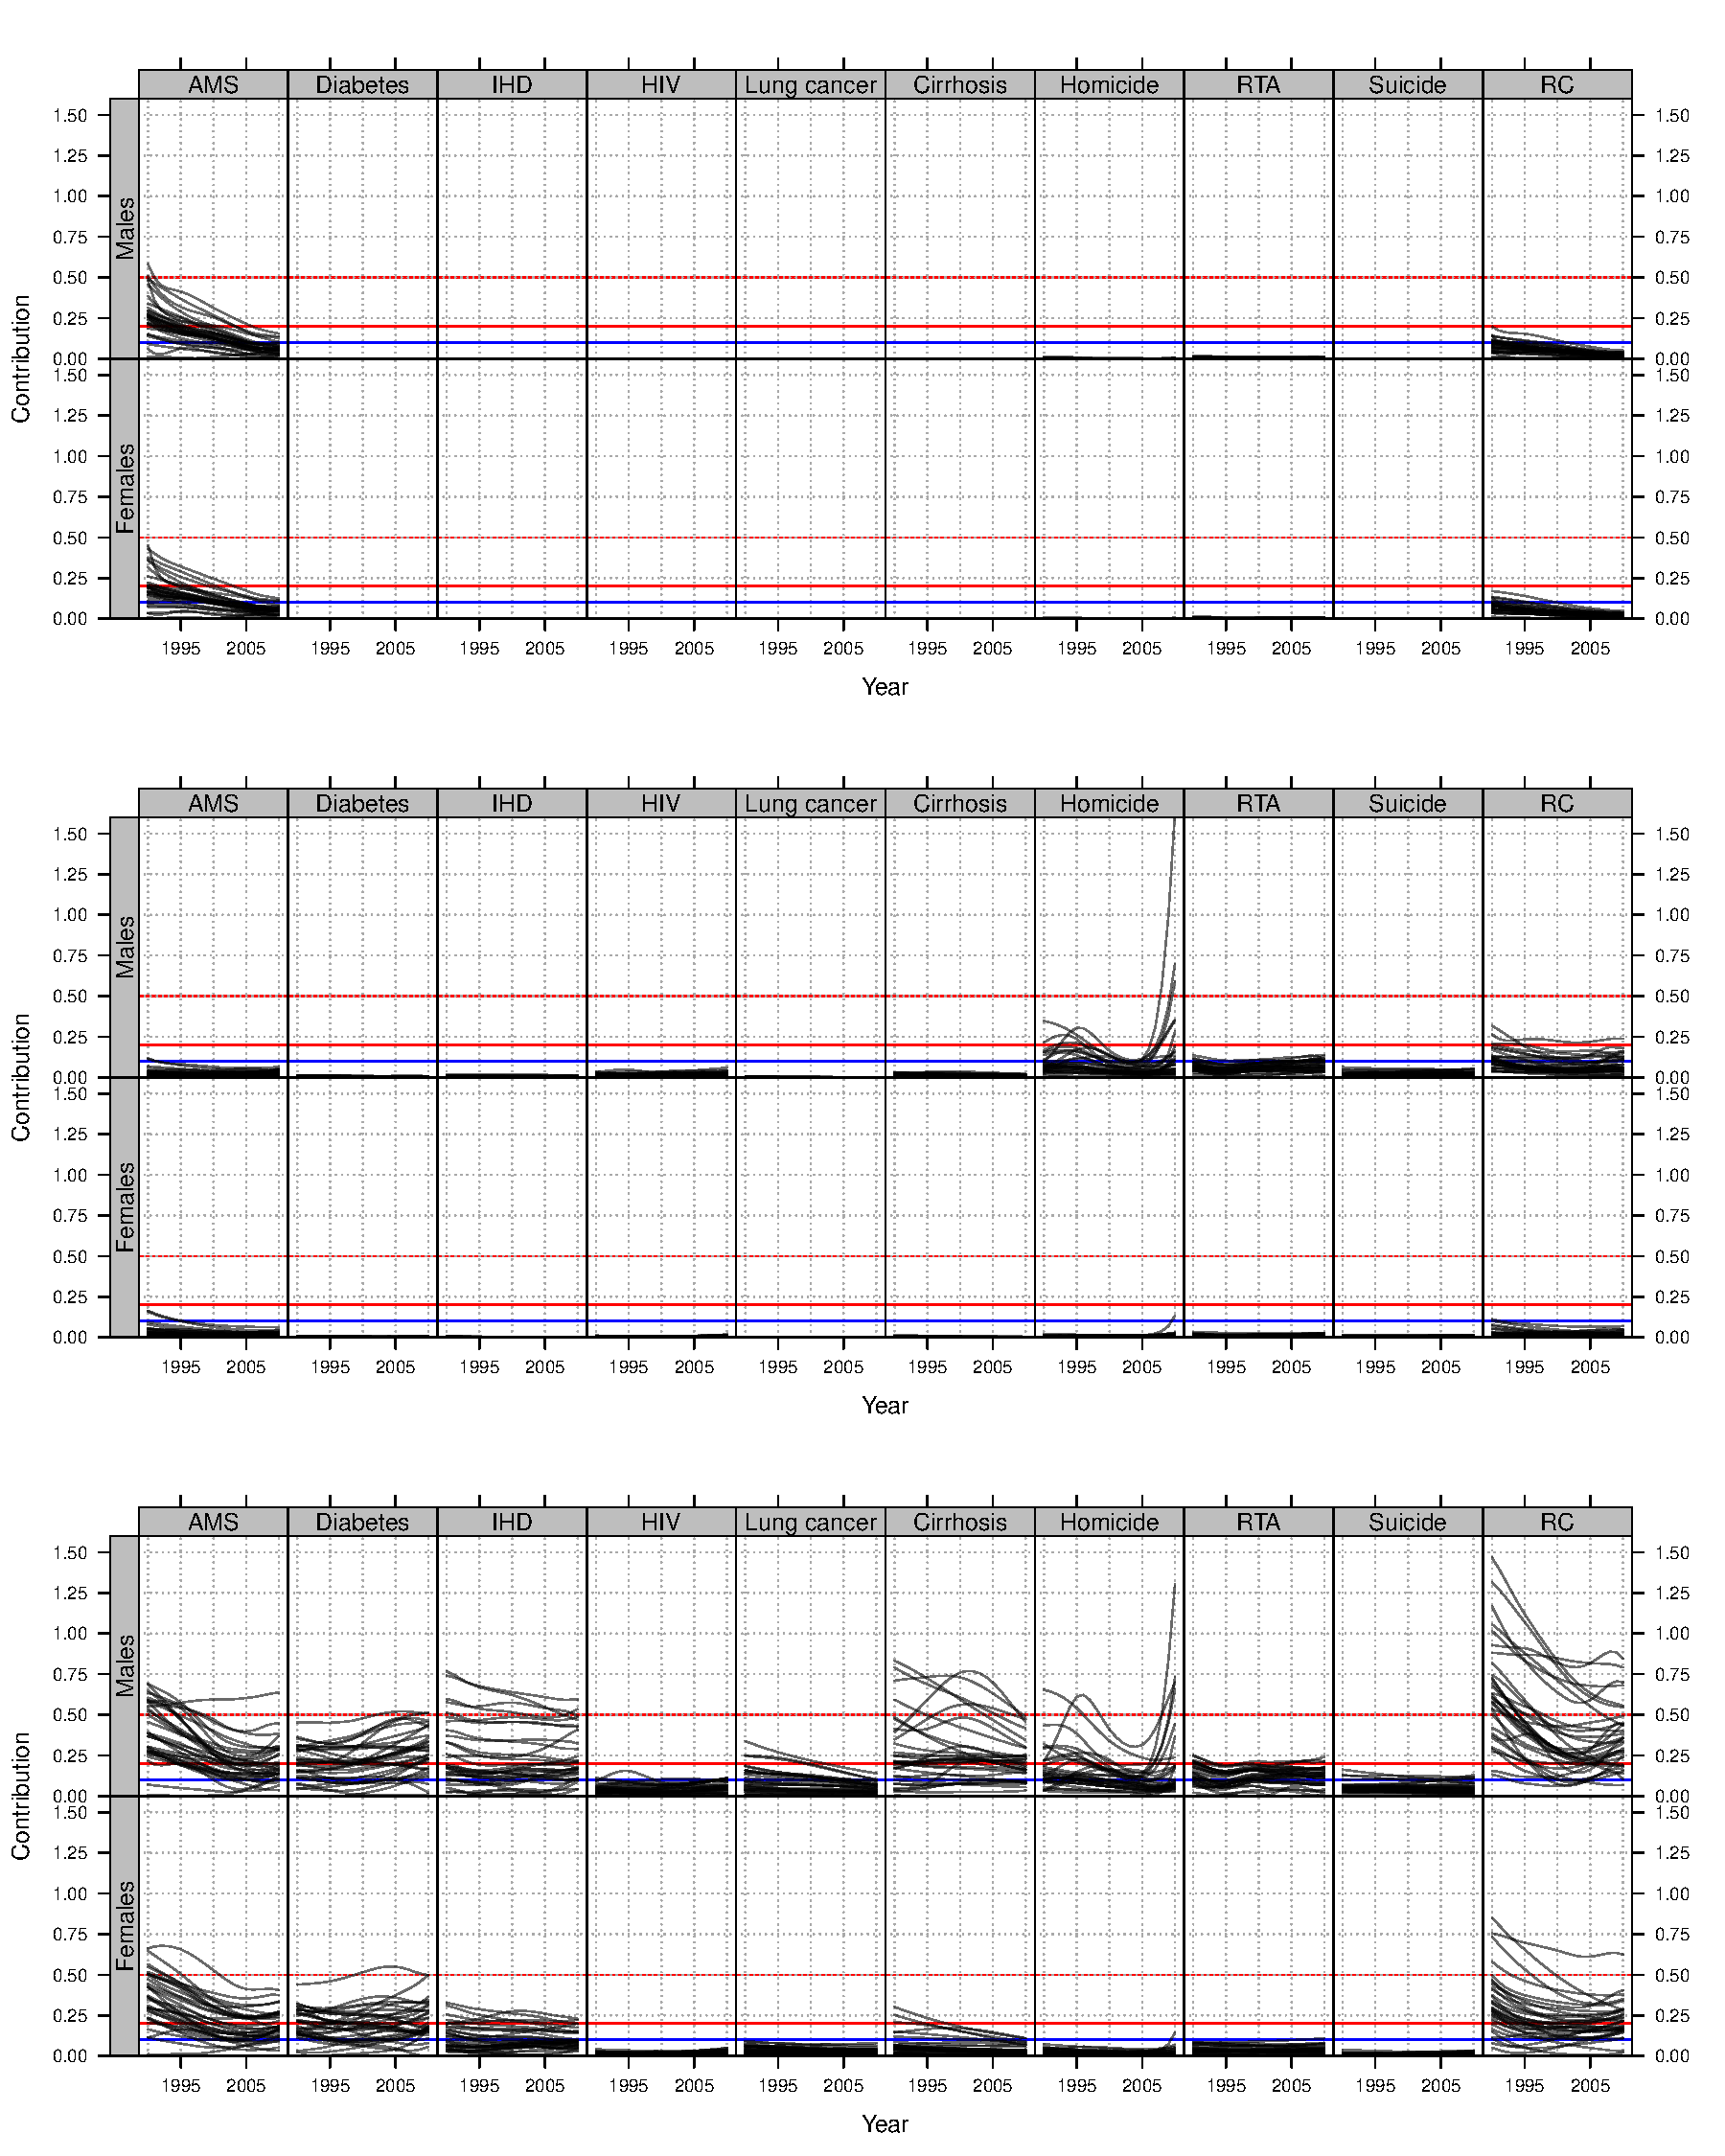
\includegraphics[scale=.4]{Figures/TLE_Decomp.pdf}
%Source: own calculations based on INEGI and SOMEDE
%\end{figure}


%This will show a few small multiples figures, tbd 

%\section*{Discussion}
%Talk about the role of homicide and other major causes. How many years of life
%were lost? (not just expectancy). maybe..

\section*{Discussion}
\subsection*{Child and young-adult mortality}

This analysis demonstrates the potential contribution of achieving the low mortality benchmark to improvements in survival. However, it is concerning that the low mortality benchmarks have not been steadily increasing over the period studied. Trends were flat for children, they are experiencing almost full survival before age 15. More worrisome is the common shift after 2005 in adults aged 15-39 and decreasing survival among older adults aged 35-74.

Despite the flattening pattern of the low mortality benchmark in children, our results show that all states in Mexico have improved survival towards this benchmark and to the maximum survival. Causes amenable to medical service are at the heart of such improvements, consistent with decreases in infectious and respiratory diseases associated with public health interventions targeted to children in Mexico previously documented \citep{sepulveda2006}. For example, Puebla and Tlaxcala improved survival over half a year since the 1990's. By 2010 survival was improved so that all states' temporary life expectancy ranged between 14.6 and 14.8 years. We further estimated survival inequalities between states by age group calculating Gini coefficients for every year (Figure \ref{fig:Gini}).  Indeed, survival equality before age 15 is almost achieved paralleling improvements in mortality rates during the period. In addition, our results are also consistent with advances in coverage for skilled attendance at delivery, which by 2012 remained above 90\% and more than 78\% of children under age one visited the doctor to monitor their development and growth  \citep{urquieta2015evolution}. Moreover, vaccination coverage has been achieved for the entire young population, the success of such public health interventions are in line with our results, underscoring the improvements in survival in the population younger than 15 years associated to the progress detected in health insurance coverage due to vaccination programs and the implementation of the Seguro Popular \citep{urquieta2015evolution}. Although average years lived below 15 has improved, there still exist areas of opportunity to achieve full-survival under age 15 in causes amenable to medical service, mainly in states in the Central and Southern regions of the country. 


\subsection*{Older-adult mortality}

Adults aged 15-39 show a converging pattern towards the low mortality benchmark in all states just until 2005. A sudden increase in homicide rates widened the gap with the low mortality benchmark by almost four times on average in 2010 relative to the level observed in 2005. Previous research documented losses in the overall life expectancy up to three years in the state of Chihuahua (the bordering state with Texas, USA) and almost two years in Sinaloa, Durango (North) and Guerrero (South) between 2005 and 2010 due to homicides \citep{Aburto2015}. Our findings show that the trend towards the low mortality benchmark was reversed after 2005 due to the increase in homicide mortality, with a peak in 2011. Although homicide rates decreased after 2011, they still are the main cause of death contributing to the gap between the observed survival and the low mortality benchmark in particular states, such as Sinaloa, Durango in the North, Nayarit and Michoac\'an in the cetral region, and Guerrero in the South. These findings underscore the need for effective interventions to reduce homicide mortality, as it still contributes the most to survival shortcomings among the young-adult population and mortality inequality among states. Even ten years after the national security strategy that aimed at reducing drug cartels' operations started and homicides begun to spread all over the country \citep{espinal2015analysis}, the effect of homicide on average survival is appalling. Between-state inequality in female survival was much smaller over the same period (figure \ref{fig:Gini}), though females showed the same overall trend of convergence, followed by divergence after 2005. 


%rember capital letters to norht, south, etc..
In Mexico, since the beginning of the 1990's, adult survival in ages 40-74 deteriorate for males and stagnate for females. Our results help explain on this pattern showing that the low mortality benchmark decreased as a result of state-specific mortality trends and the interaction between specific causes of death. In particular, there are offsetting effects between improvements in causes amenable to medical service, such as infectious and respiratory diseases, and deterioration in diabetes, isquemic heart diseases (IHD), and behavior-related mortality through cirrhosis and homicides. 

Out of 35 potential years, adult females in Mexico are living less than 33 and males less than 31 since the 1990's. The increase in  diabetes, IHD and cirrhosis mortality is at the heart of survival's deterioration, with clear regional variations. Although improvements in causes amenable to medical service were witnessed, almost every state still has potential to improve in this ages, in particular the Northern states of Sonora, Chihuahua and Baja California. Diabetes mortality increased over the period and contributed to increases in the gap to achieve the low mortality benchmark. Diabetes-related mortality increased 23\% from 1998 to 2002, and the prevalence of diabetes was estimated at 14.4\% in the adult population in 2006. These figures underscore the emerging epidemic of diabetes \citep{glassman2010confronting}. To put this in perspective, Coahuila, the state of Mexico, Guanajuato, the Federal District, Tabasco and Puebla could increase survival by almost one year if diabetes mortality were to achieve the low mortality benchmark. Similarly, mortality related to IHD contributes to lowering life expectancy in adults. There is a clear regional pattern in the country. Almost all the states in the Northern region could potentially benefit with one additional year in life expectancy if the low mortality benchmark were reached, where as the Central and Southern regions present a lower impact of IHD. Cirrhosis-related mortality shows a higher impact in the Southern and Central states of the country, particularly in Quer\'etaro, M\'exico state, Hidalgo (central area) and Puebla and Oaxaca in the South. Both diabetes and IHD mortality are closely related to obesity prevalence, previous research anticipated that the increasing levels of obesity in Mexico could compromise gains in life expectancy \citep{monteverde2010obesity}. These regional differences on cause-specific mortality led to increases in health inequalities in adults aged 30-74 after 2006 for males and stagnation among females (figure \ref{fig:Gini}). 


There is still potential for improvements to reduce state-mortality differences and improve the survival among the adult population in Mexico. Several screening and prevention strategies (e.g. PREVENIMSS) for early diabetes and hypertension have been implemented in the country. However, as previous research has found, they are far from achieving the ultimate goal and including the entire population \citep{castro2010potential}. In addition, \citet{behrman2013health} show that the conditional cash transfer program PROSPERA improves health significantly for adult women older than 50. The authors also noted that the effect on men's health is much lower. They argue that this could be the result of the lack of inclusion of men in the program and the main role of women in the program's requirements. Women are recipients of the monetary transfers and they are more likely to attend clinic visits and follow health measures given by doctors in these clinics than men.

\begin{figure}
\centering
\caption{Survival inequality by age group and sex, 1990-2010.}
\label{fig:Gini}
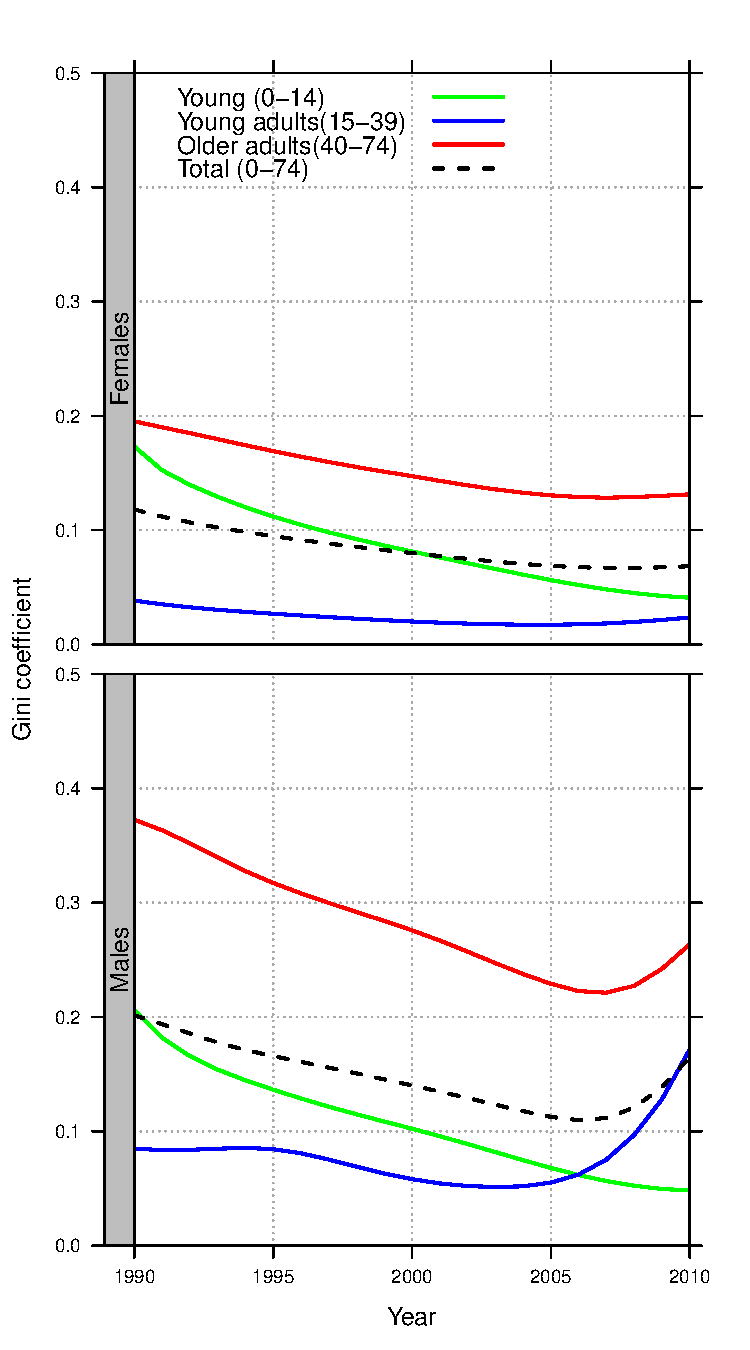
\includegraphics[scale=.5]{Figures/Gini_fig.pdf}

 Source: calculations based on INEGI and SOMEDE files.
\end{figure}



\subsection*{Conclusion}
Improving health is a priority for governments of many developing countries. In part to reduce child mortality, improve maternal health and lessen the impact of other infectious diseases, such as HIV/AIDS, to achieve the Millennium Development Goals established for 2015 \citep{united2009millennium}.  Mexico has succeeded in reducing mortality and inequalities in children and the young population. Nevertheless, our results show that older adults are becoming a vulnerable group, and more efforts are required to reduce the burden of conditions amenable to health services and policy-related conditions. In particular, this group lacks comprehensive interventions to reduce the burden of violence through homicides, chronic-degenerative
causes of death, such as diabetes and IHD, and behavior-related conditions such as cirrhosis.  

There is no simple way to lessen the impact of such conditions, but it is clear that new approaches are needed to improve survival in the adulthood and to minimize health disparities between states. Preventing diabetes and IHD implies fundamental political challenges. Therefore,  public health initiatives should focus in health care for chronic conditions as recently suggested by \citet{knaul2015achieving}, but they should also influence the population towards improving health behavior. Our results reinforce the need of such, among others public health interventions, with an special focus on older adults in the Mexico. 


\end{spacing}

\section*{Competing interest}
None to declare.

%However, they still remain the world's most unequal countries \citep{Barreto2012}.
%}
%\bibliographystyle{plainnat}
\newpage
 \bibliography{AburtoRiffe_Bib.bib}
 
 
 \newpage
\section*{Supplemental material}
Appendix Table 1. Definitions of cause-of-death categories using the \nth{9} and \nth{10} revision of the International Classification of Diseases.\\

{\renewcommand{\baselinestretch}{1}\selectfont

\begin{longtable}{p{8cm}p{4cm}p{4cm}ccc}
\hline
\textbf{Category} & \textbf{ICD-10} & \textbf{ICD-9}\\
\hline
\endfirsthead
\multicolumn{3}{c}%
{\tablename\ \thetable\ -- \textit{Continue}} \\
\hline
\textbf{Category} & \textbf{ICD-10} & \textbf{ICD-9}\\
\hline
\endhead
\hline \multicolumn{3}{r}{\textit{Continues}} \\
\endfoot
\hline
\endlastfoot
\multicolumn{3}{l}{\bf I. Amenable to medical service}  \\
 I.A. AM-Infectious \& respiratory diseases : intestinal infections, tuberculosis, zoonotic bacterial diseases, other bacterial diseases, septicemia, poliomyelitis, measles, rubella, infectious hepatitis, ornithosis, rickettsioses/ arthropod-borne, syphilis (all forms), yaws, respiratory diseases, influenza \& pneumonia, chronic lower respiratory diseases & A00-A09, A16-A19, B90, A20-A26, A28, A32, A33, A35, A36, A37, A40-A41, A80, B05-B06, B15-B19, A70, A68, A75, A77, A50-A64, A66, J00-J08, J20-J39, J60-J99, J09-J18, J40-J47 & 001-009, 010-018, 32, 33, 37, 137, 020-027, 38, 45, 55-56, 70, 73, 080-082, 087, 090-099, 102, 460-479, 500-519, 480-488, 490-496 \\
           I.B. AM-Cancers: malignant neoplasm of colon, skin, breast, cervix, prostate, testis, bladder, kidney-Wilm's tumor only, eye, thyroid carcinoma, Hodgkin’s disease, leukemia & C16,C18-C21, C43-C44, C50, C53, C61, C62, C67, C64, C69, C73, C81, C91-C95 & 153-154, 172-173, 174, 180, 185, 186, 188-189, 190, 193, 201, 204-208\\
           I.C. AM-Circulatory: active/acute rheumatic fever, chronic rheumatic heart disease, hypertensive disease, cerebrovascular disease & I00-I02, I05-I09, I10-I13, I15, I60-I69 & 390-392, 393-398, 401-405, 430-438\\
          I.D. AM-Birth: maternal deaths (all), congenital cardiovascular anomalies, perinatal deaths (excluding stillbirths) & O00-O99, Q20-Q28, P00-P96 & 630-676, 745-747, 760-779\\
          I.E. AM-Other: disease of thyroid, epilepsy, peptic ulcer, appendicitis, abdominal hernia, cholelithiasis \& cholecystitis, nephritis, benign prostatic hyperplasia, misadventures to patients during surgical or medical care, cisticerchosis & E00-E07, 40-G41, K25-K27, K35-K38, K40-K46, K80-K81,  N00-N07, N17-N19, N25-N27, N40, Y60-Y69, Y83-Y84, B69 & 240-246, 345, 531-533, 540-543, 550-553, 574-575.1, 580-589, 600, E870-E876, E878-E879\\
 & \\          
 {\bf II. Diabetes}  & E10-E14 & 250 \\      
 & \\
 {\bf III. Ischemic Heart Diseases (IHD)}   & I20-I25 & 410-414, 429.2\\
 & \\           
 {\bf IV. HIV/AIDS} & B20-B24 & 279.1, 042-044\\ 
  & \\                
{\bf V. Lung cancer}  & C33-C34 & 162\\
  & \\          
{\bf VI. Cirrhosis}&  K70 & 571.1-571.3\\
 & \\          
{\bf VII. Homicides}  & X85-Y09 & E960-E969\\     
 & \\           
 {\bf VIII. Road traffic accidents}  & V01-V99 & E810-E819 \\     
 & \\           
{\bf IX. Suicide and self-inflicted injuries}  & U03, X60-X84, Y87.0 & E950-E959\\ 
 & \\          
{\bf X. Residual Causes }:  other cancers and other heart diseases & C00-D48, I00-I99 if not listed above, R00-R99 & 140-239, 390-459 if not listed above, 780-799
\label{ME_Mex}
\end{longtable}

\begin{figure}
\centering
\caption{Cause-specific mortality counts, 1990-2010.}
\label{fig:ClassSens}
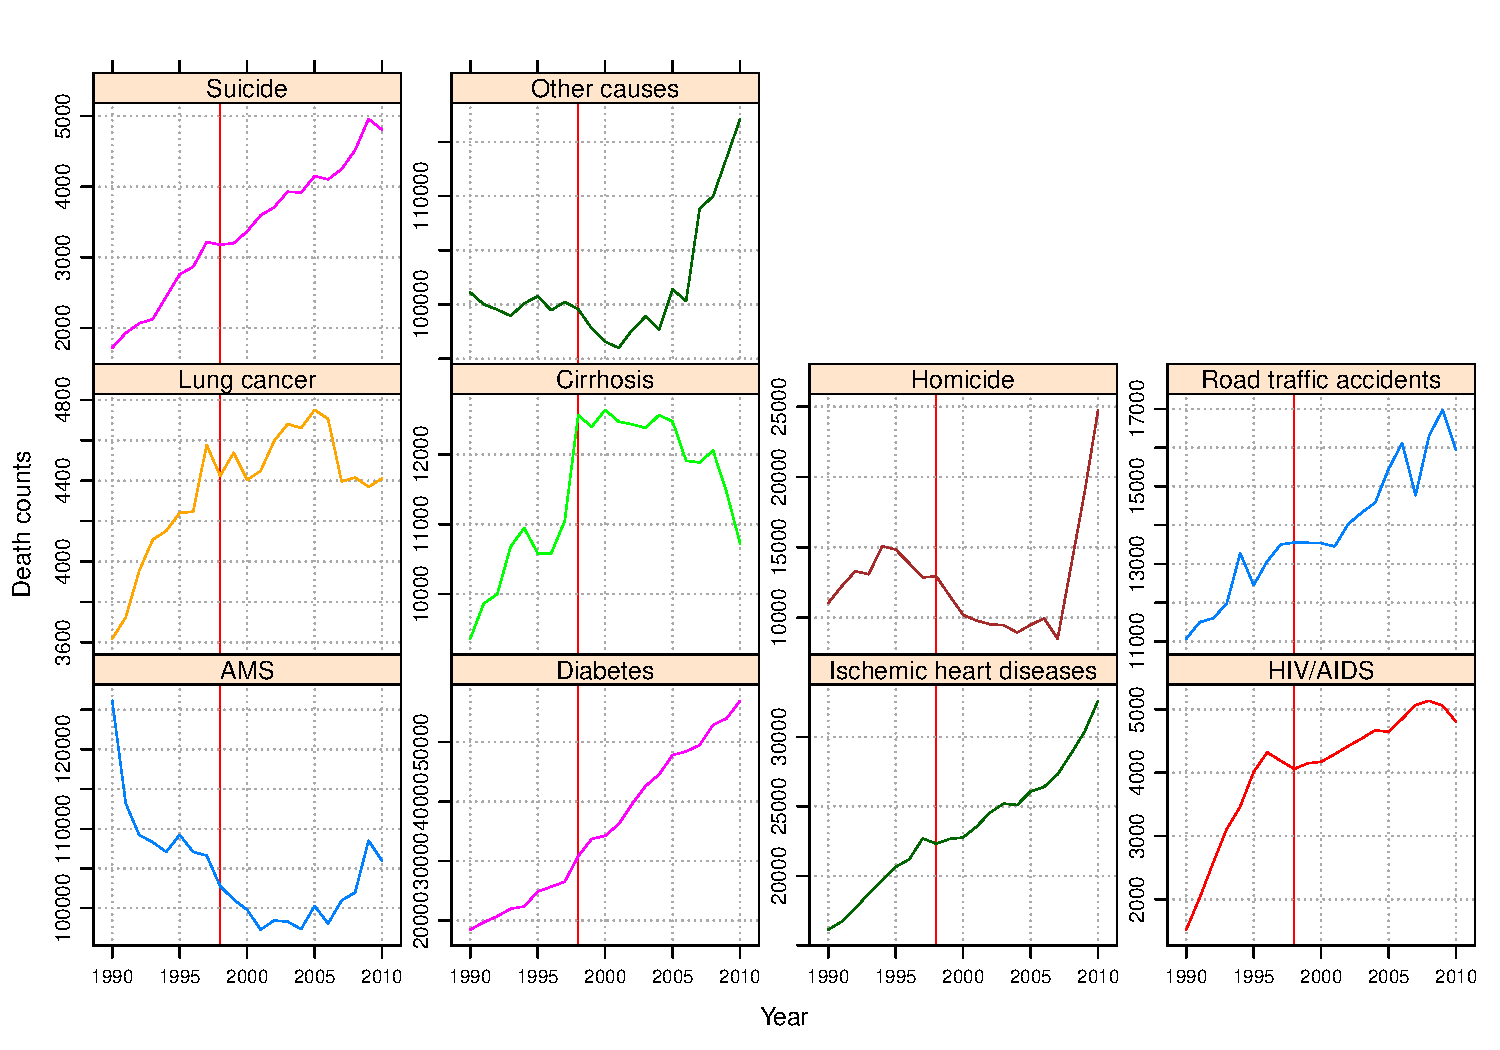
\includegraphics[scale=.6]{Figures/Class_fig.pdf}

Note: AMS ``amenable to medical service''. The red line indicates the change in ICD revision. Source: INEGI files. 
\end{figure}



\subsection*{Temporary Life Expectancy}
Temporary life expectancy between ages
$x_1$ and $x_2$, for $x_1<x_2$, is defined as the average years of life lived between these ages according to a given set of mortality rates \citep{arriaga1984}. We denote this quantity as
$e(x_1,x_2)$, and its benchmark minimum as $e^{\star}(x_1,x_2)$. Defined in
terms of lifetable survivorship, $\ell(x)$:

\begin{equation}
e(x_1,x_2) = \frac{\int _{x_1}^{x_2} \ell(x) \dd x}{\ell(x_1)}
\end{equation}

If full survival is achieved, the maximum life expectancy is $x_2-x_1$.  For example, if we set $x_1=0$ and $x_2=14$, if no person dies between the ages 0 and 14, on average the population lives 14 full years.


\begin{figure}
\centering
\caption{Cause-specific contributions to state differences from low mortality benchmark for male young people, 1990-2010.}
\label{fig:e0_14_males}
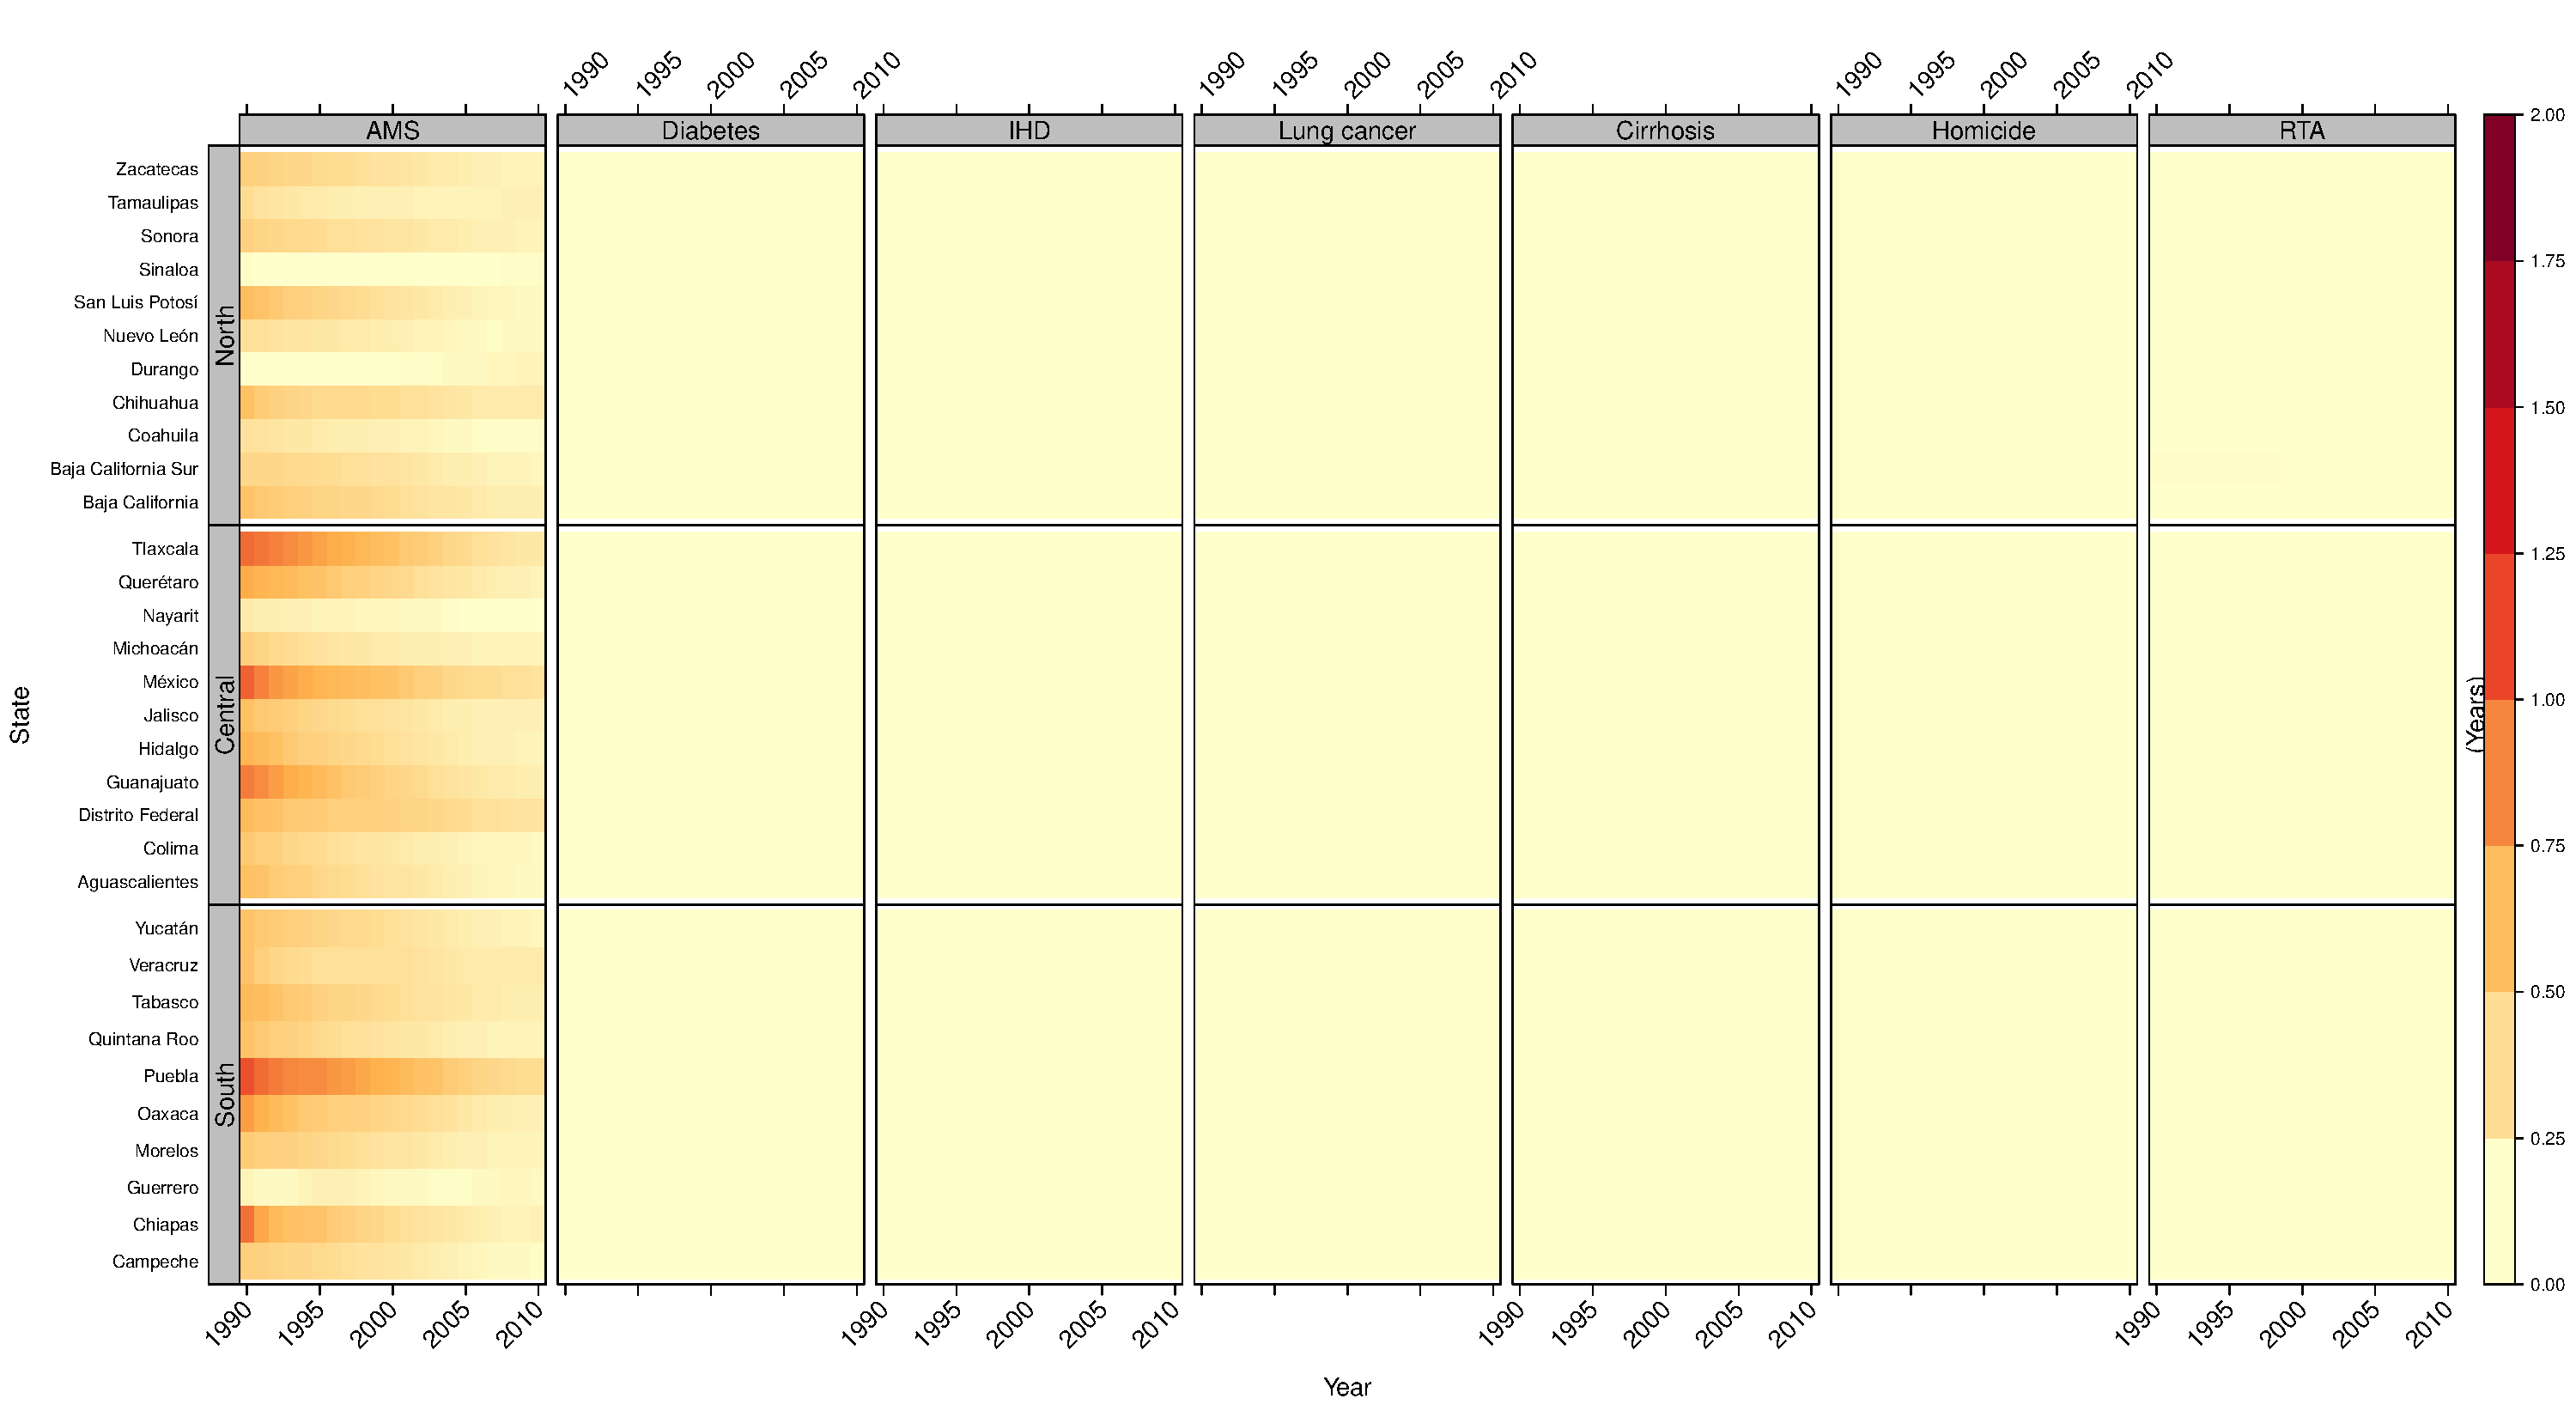
\includegraphics[scale=.3]{Figures/Young_Male_heatmap.pdf}
Note: Note: AMS is ``amenable to medical service'', IHD is ``isquemic heart diseases'', and RTA is ``road traffic accidents''. Source: calculations based on INEGI and SOMEDE files. \end{figure}

\begin{figure}
\centering
\caption{Cause-specific contributions to state differences from low mortality benchmark for female young people, 1990-2010.}
\label{fig:e0_14_females}
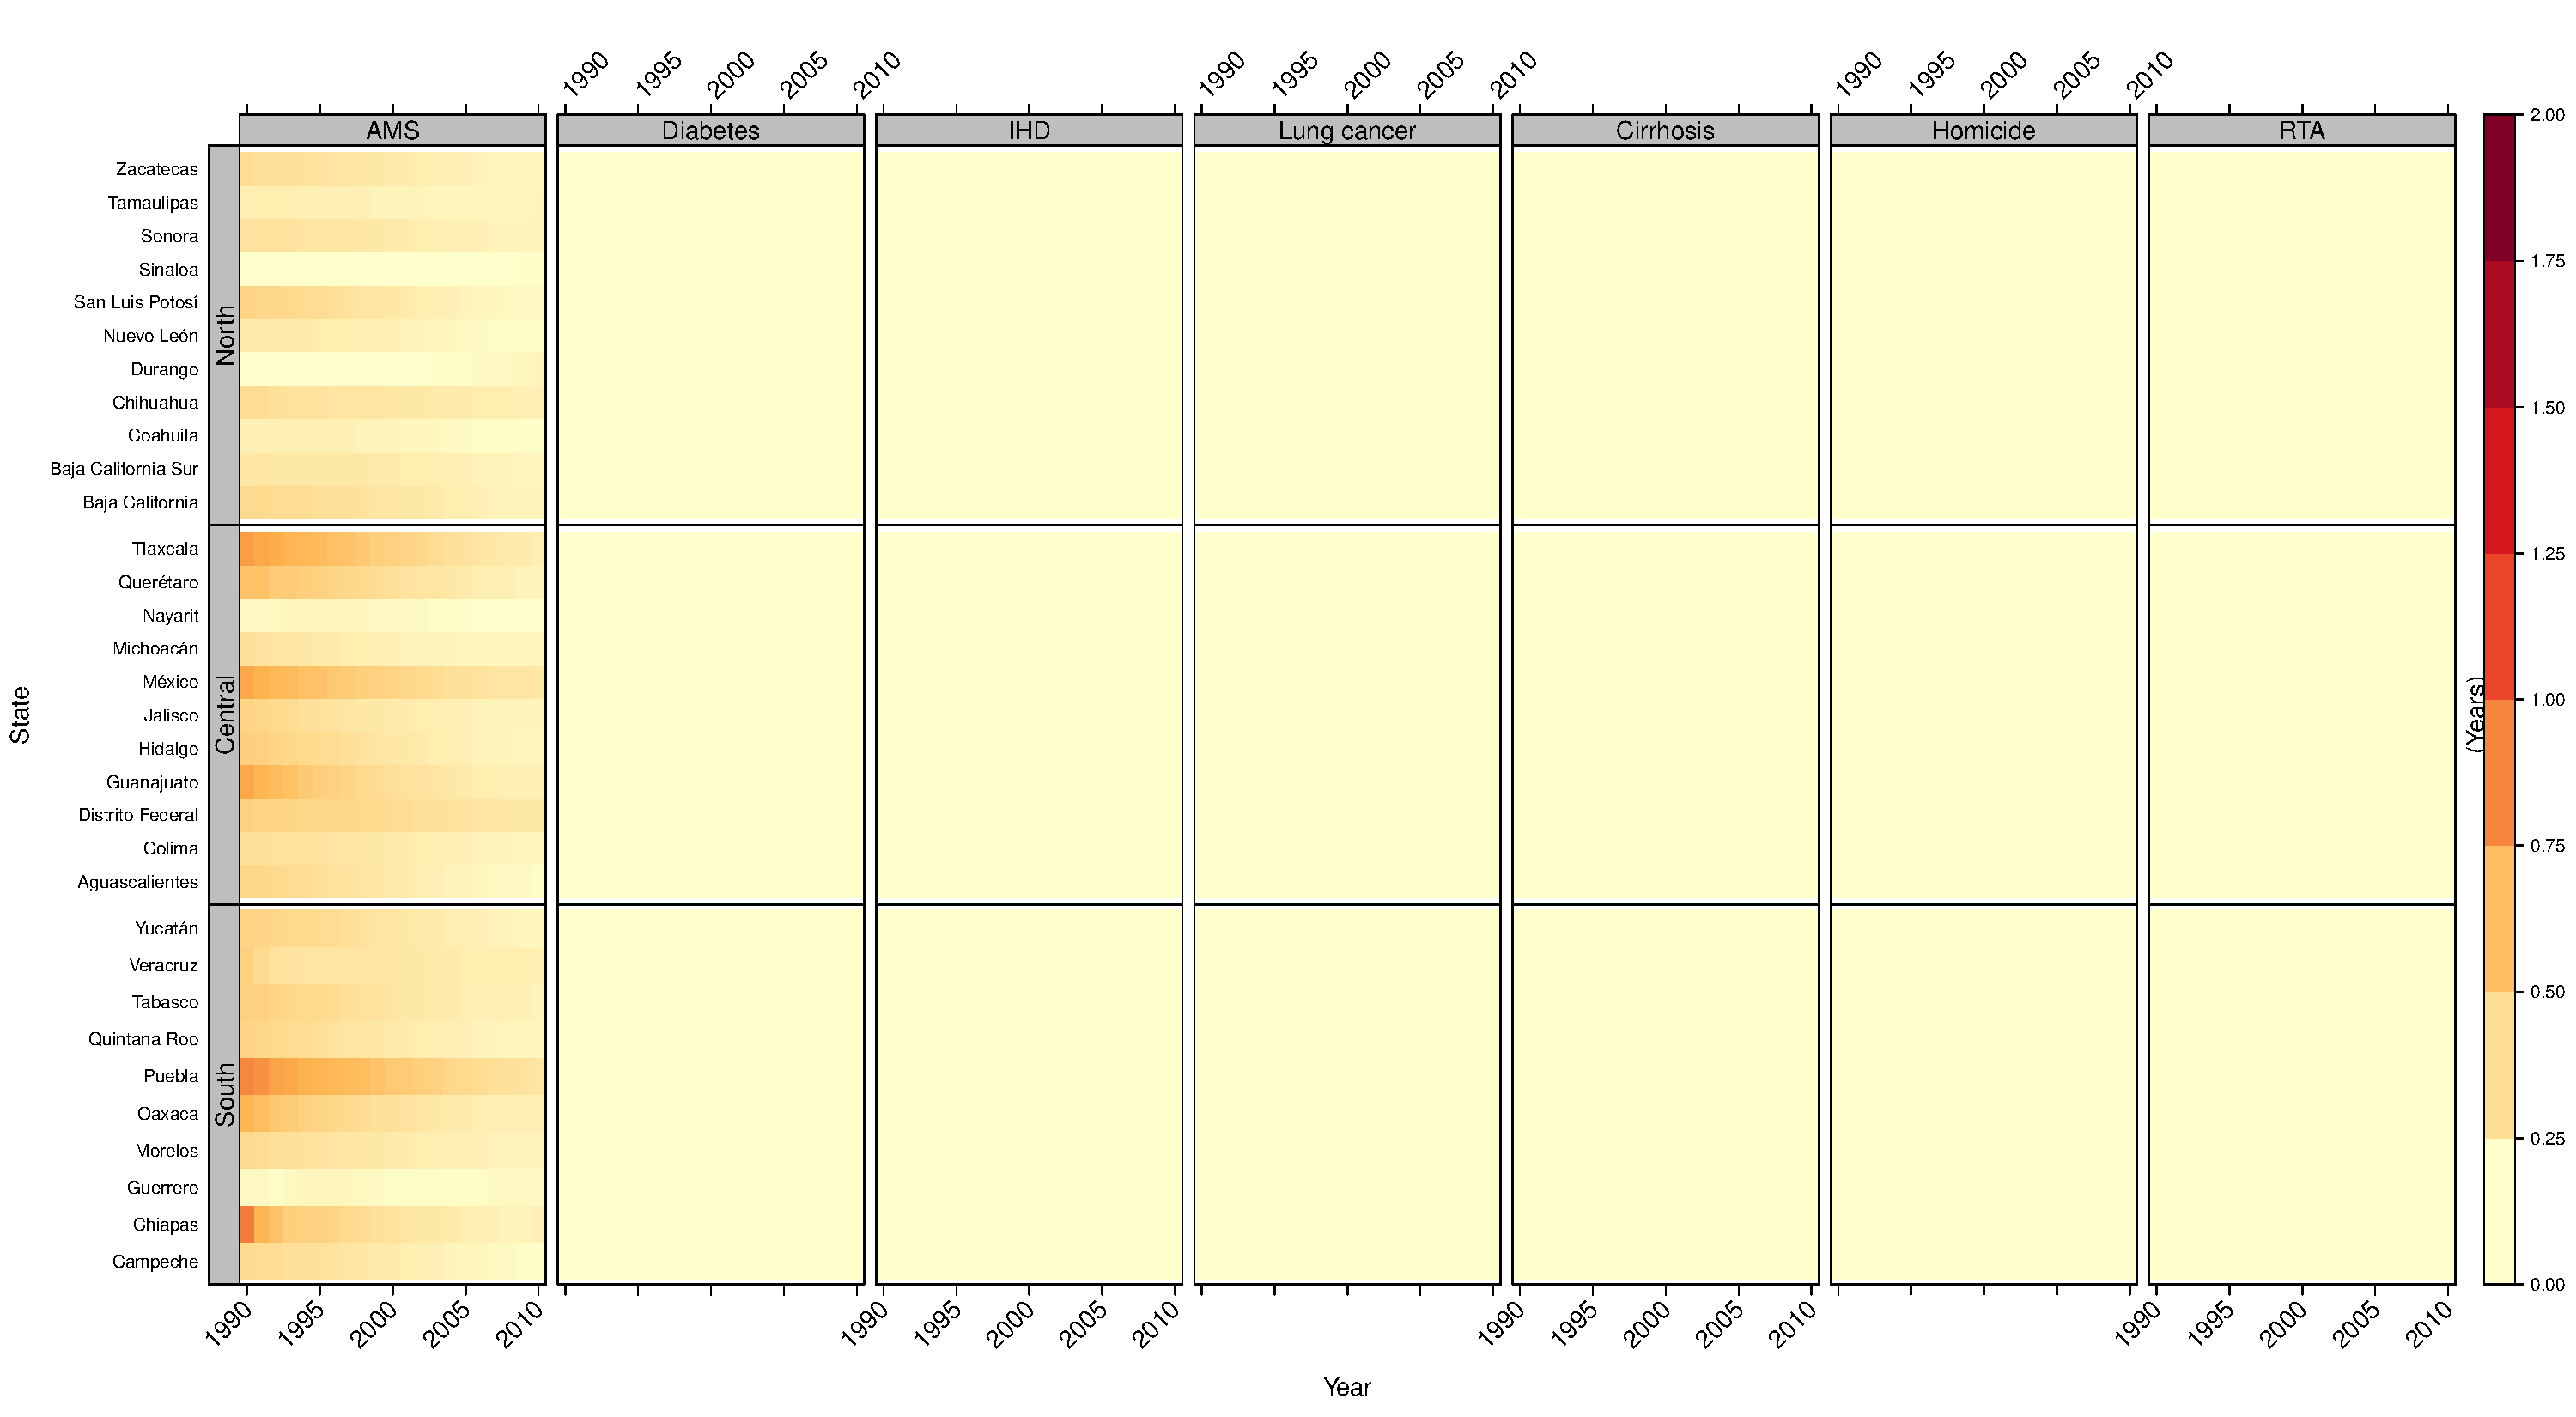
\includegraphics[scale=.3]{Figures/Young_Female_heatmap.pdf}
Note: AMS is ``amenable to medical service'', IHD is ``isquemic heart diseases'', and RTA is ``road traffic accidents''. Source: calculations based on INEGI and SOMEDE files. \end{figure}



\begin{figure}
\centering
\caption{Cause-specific contributions to state differences from low mortality benchmark for male young adults, 1990-2010.}
\label{fig:e15_39_males}
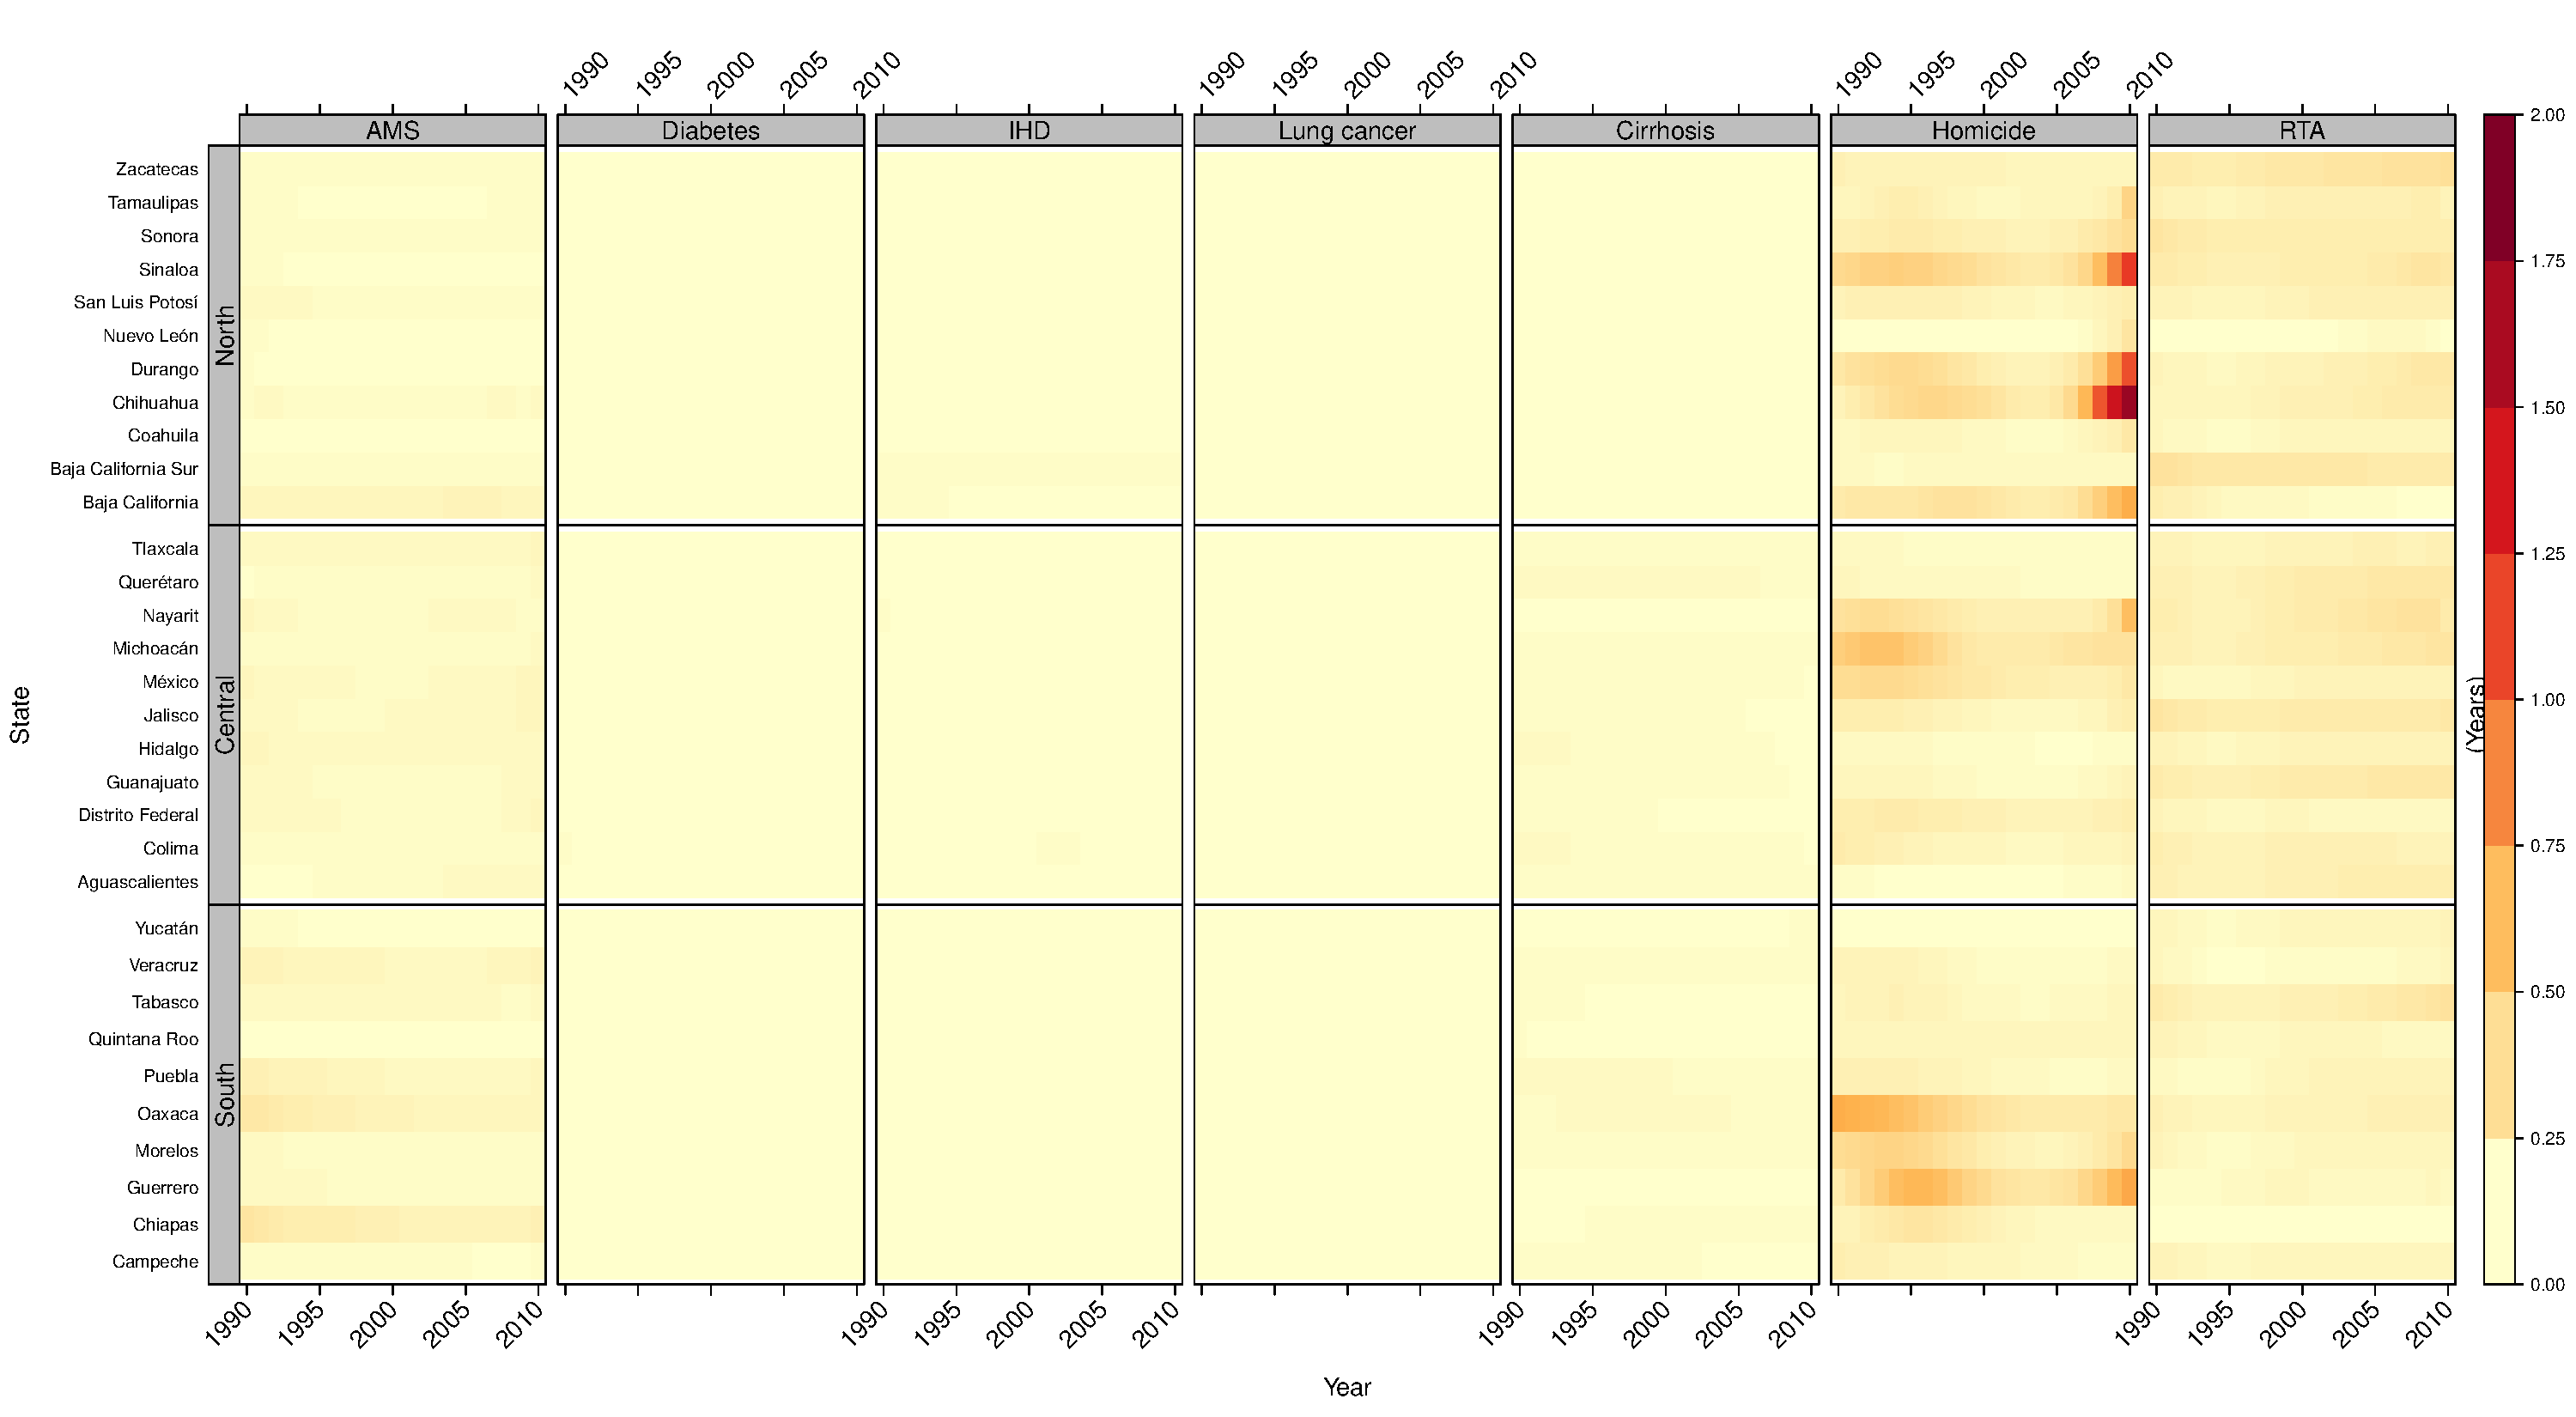
\includegraphics[scale=.3]{Figures/YoungAdult_Male_heatmap.pdf}
Note: AMS is ``amenable to medical service'', IHD is ``isquemic heart diseases'', and RTA is ``road traffic accidents''. Source: calculations based on INEGI and SOMEDE files.
\end{figure}

\begin{figure}
\centering
\caption{Cause-specific contributions to state differences from low mortality benchmark for female young adults, 1990-2010.}
\label{fig:e15_39_females}
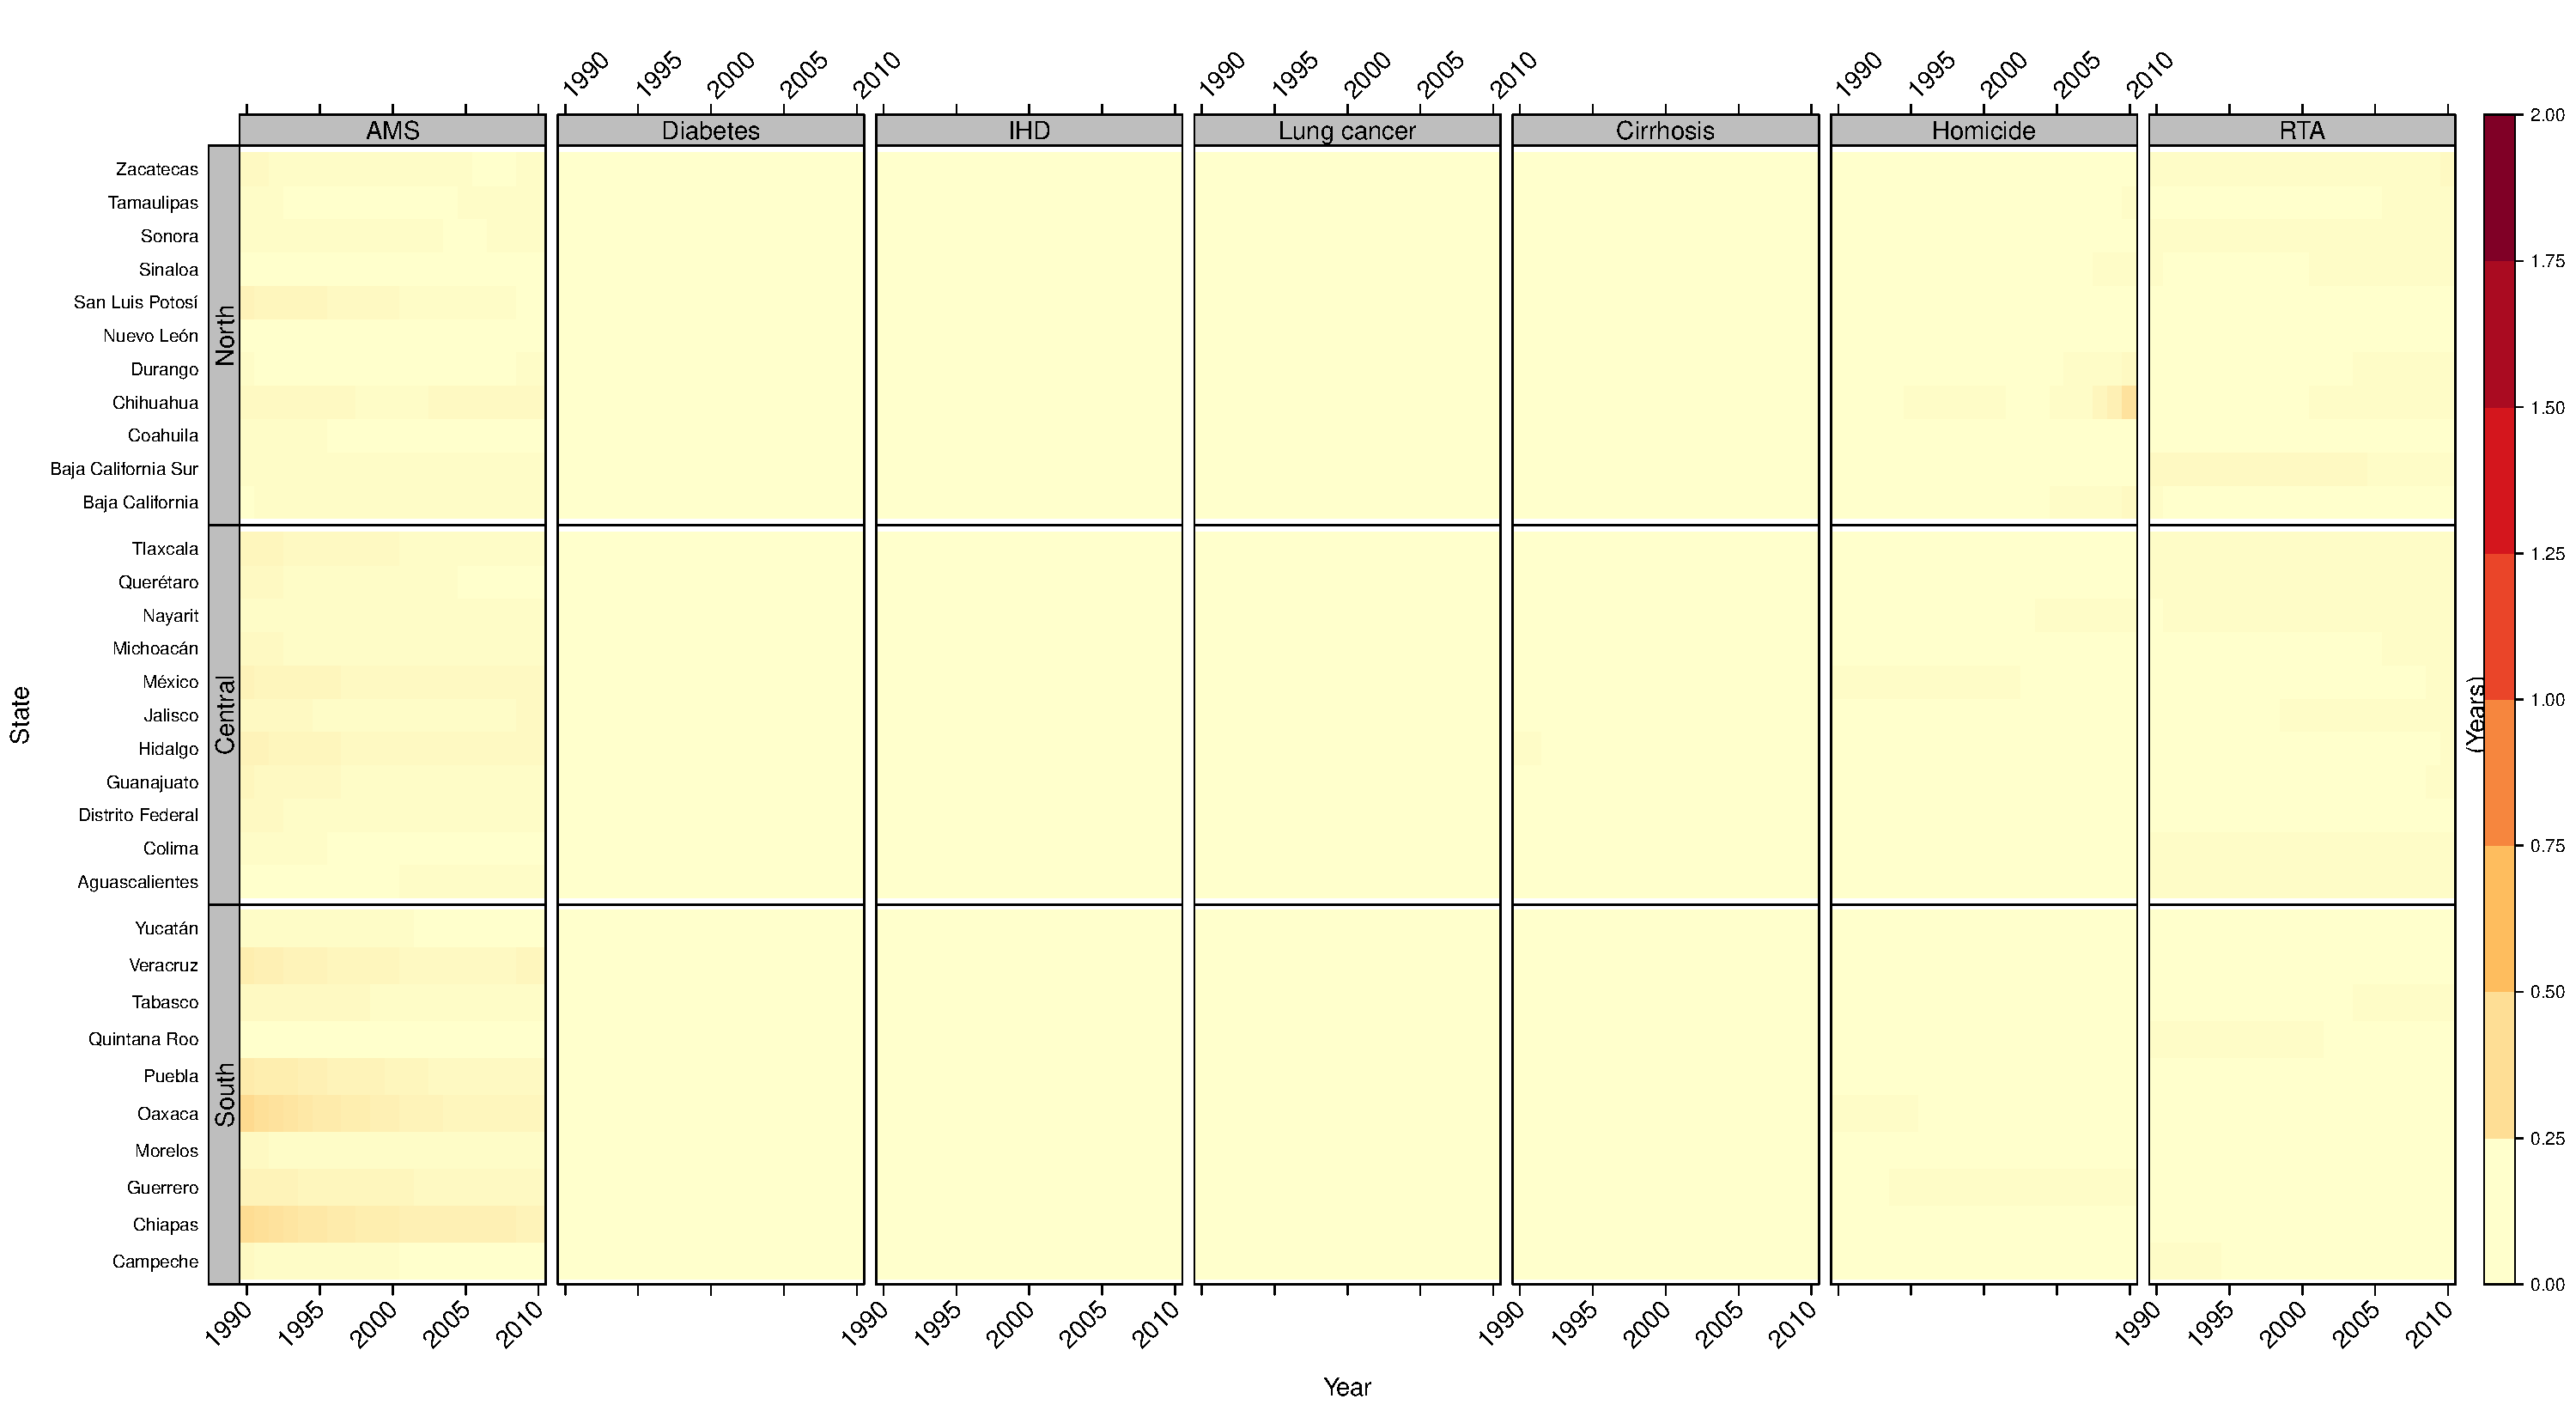
\includegraphics[scale=.3]{Figures/YoungAdult_Female_heatmap.pdf}
Note: AMS is ``amenable to medical service'', IHD is ``isquemic heart diseases'', and RTA is ``road traffic accidents''. Source: calculations based on INEGI and SOMEDE files.
\end{figure}



\begin{landscape}

% latex table generated in R 3.2.2 by xtable 1.8-0 package
% Wed Feb  3 15:51:09 2016
\begin{table}[ht]
\caption{Selected cause-specific contributions to deviations from low mortality benchmark, male older-adults by state and years, 2000, 2005 and 201}
\rowcolors{1}{}{lightgray}
\begin{footnotesize}
\centering
\begin{tabular}{lllll|lll|lll|lll|lll|lll}
\hline
Region & State &  \multicolumn{3}{c}{Amenable to M.S} & \multicolumn{3}{c}{Diabetes} &  \multicolumn{3}{c}{IHD} &  \multicolumn{3}{c}{Lung cancer}&  \multicolumn{3}{c}{Cirrhosis}&  \multicolumn{3}{c}{Homicide}\\
  \hline
& Year  & 2000 & 2005 & 2010 & 2000 & 2005 & 2010 & 2000 & 2005 & 2010 & 2000 & 2005 & 2010 & 2000 & 2005 & 2010 & 2000 & 2005 & 2010 \\ 
  \hline
  
North & Baja California & 0.59 & 0.6 & 0.64 & 0.3 & 0.29 & 0.28 & 0.62 & 0.55 & 0.47 & 0.1 & 0.08 & 0.06 & 0.12 & 0.1 & 0.09 & 0.16 & 0.12 & 0.44 \\ 
   & Baja California Sur & 0.26 & 0.22 & 0.21 & 0.22 & 0.19 & 0.16 & 0.46 & 0.45 & 0.42 & 0.22 & 0.18 & 0.14 & 0.18 & 0.17 & 0.16 & 0.08 & 0.07 & 0.06 \\ 
   & Coahuila & 0.4 & 0.32 & 0.3 & 0.38 & 0.48 & 0.42 & 0.49 & 0.47 & 0.49 & 0.11 & 0.09 & 0.07 & 0.1 & 0.09 & 0.09 & 0.03 & 0.02 & 0.08 \\ 
   & Chihuahua & 0.47 & 0.4 & 0.45 & 0.22 & 0.25 & 0.3 & 0.57 & 0.54 & 0.49 & 0.12 & 0.1 & 0.09 & 0.2 & 0.18 & 0.17 & 0.17 & 0.13 & 1.3 \\ 
   & Durango & 0.22 & 0.2 & 0.16 & 0.2 & 0.23 & 0.23 & 0.24 & 0.3 & 0.41 & 0.09 & 0.08 & 0.06 & 0.09 & 0.1 & 0.08 & 0.14 & 0.13 & 0.65 \\ 
   & Nuevo Le\'on & 0.32 & 0.28 & 0.31 & 0.17 & 0.2 & 0.26 & 0.52 & 0.48 & 0.53 & 0.12 & 0.09 & 0.07 & 0.02 & 0.03 & 0.03 & 0 & 0 & 0.09 \\ 
   & San Luis Potos\'i & 0.16 & 0.1 & 0.08 & 0.12 & 0.17 & 0.23 & 0.09 & 0.1 & 0.11 & 0.04 & 0.04 & 0.04 & 0.23 & 0.21 & 0.16 & 0.1 & 0.06 & 0.09 \\ 
   & Sinaloa & 0.17 & 0.14 & 0.14 & 0.12 & 0.1 & 0.02 & 0.34 & 0.35 & 0.32 & 0.2 & 0.15 & 0.1 & 0 & 0 & 0 & 0.22 & 0.14 & 0.73 \\ 
   & Sonora & 0.46 & 0.39 & 0.39 & 0.21 & 0.19 & 0.17 & 0.64 & 0.61 & 0.59 & 0.19 & 0.14 & 0.1 & 0.08 & 0.07 & 0.08 & 0.09 & 0.09 & 0.18 \\ 
   & Tamaulipas & 0.28 & 0.23 & 0.29 & 0.31 & 0.33 & 0.37 & 0.46 & 0.44 & 0.43 & 0.13 & 0.1 & 0.07 & 0.07 & 0.06 & 0.05 & 0.06 & 0.06 & 0.18 \\ 
   & Zacatecas & 0.16 & 0.14 & 0.16 & 0.08 & 0.11 & 0.15 & 0.09 & 0.08 & 0.1 & 0.07 & 0.06 & 0.05 & 0.08 & 0.08 & 0.08 & 0.1 & 0.08 & 0.06 \\ 
  Central & Aguascalientes & 0.21 & 0.19 & 0.2 & 0.3 & 0.3 & 0.28 & 0.15 & 0.17 & 0.17 & 0.1 & 0.08 & 0.07 & 0.22 & 0.21 & 0.21 & 0.04 & 0.04 & 0.06 \\ 
   & Colima & 0.12 & 0.1 & 0.14 & 0.19 & 0.19 & 0.21 & 0.23 & 0.22 & 0.21 & 0.12 & 0.11 & 0.09 & 0.31 & 0.27 & 0.24 & 0.16 & 0.14 & 0.18 \\ 
   & Distrito Federal & 0.34 & 0.24 & 0.37 & 0.48 & 0.52 & 0.51 & 0.34 & 0.31 & 0.29 & 0.04 & 0.03 & 0.02 & 0.27 & 0.21 & 0.16 & 0.06 & 0.04 & 0.06 \\ 
   & Guanajuato & 0.2 & 0.16 & 0.19 & 0.38 & 0.44 & 0.46 & 0.13 & 0.15 & 0.16 & 0.03 & 0.03 & 0.03 & 0.31 & 0.26 & 0.19 & 0.03 & 0.02 & 0.04 \\ 
   & Hidalgo & 0.25 & 0.17 & 0.17 & 0.16 & 0.2 & 0.25 & 0.07 & 0.13 & 0.17 & 0.02 & 0.02 & 0.01 & 0.61 & 0.51 & 0.42 & 0.06 & 0.03 & 0.03 \\ 
   & Jalisco & 0.3 & 0.27 & 0.29 & 0.29 & 0.3 & 0.3 & 0.25 & 0.24 & 0.22 & 0.07 & 0.06 & 0.04 & 0.24 & 0.22 & 0.2 & 0.07 & 0.04 & 0.09 \\ 
   & M\'exico & 0.25 & 0.2 & 0.25 & 0.39 & 0.47 & 0.51 & 0.14 & 0.12 & 0.13 & 0.01 & 0.01 & 0.01 & 0.59 & 0.47 & 0.34 & 0.15 & 0.11 & 0.1 \\ 
   & Michoac\'an & 0.16 & 0.13 & 0.15 & 0.2 & 0.26 & 0.32 & 0.11 & 0.13 & 0.15 & 0.05 & 0.04 & 0.03 & 0.21 & 0.22 & 0.23 & 0.2 & 0.2 & 0.19 \\ 
   & Nayarit & 0.14 & 0.11 & 0.1 & 0.08 & 0.08 & 0.07 & 0.19 & 0.19 & 0.17 & 0.12 & 0.09 & 0.06 & 0.07 & 0.08 & 0.08 & 0.16 & 0.15 & 0.37 \\ 
   & Quer\'etaro & 0.23 & 0.16 & 0.14 & 0.23 & 0.26 & 0.33 & 0.16 & 0.2 & 0.24 & 0.04 & 0.04 & 0.04 & 0.76 & 0.7 & 0.46 & 0.08 & 0.05 & 0.03 \\ 
   & Tlaxcala & 0.14 & 0.07 & 0.04 & 0.32 & 0.37 & 0.43 & 0.01 & 0.01 & 0 & 0.01 & 0.02 & 0.02 & 0.42 & 0.36 & 0.3 & 0.09 & 0.07 & 0.04 \\ 
  South & Campeche & 0.03 & 0.03 & 0.06 & 0.08 & 0.1 & 0.13 & 0.15 & 0.15 & 0.14 & 0.07 & 0.06 & 0.05 & 0.25 & 0.24 & 0.24 & 0.12 & 0.09 & 0.07 \\ 
   & Chiapas & 0.39 & 0.3 & 0.28 & 0.02 & 0.06 & 0.12 & 0.04 & 0.04 & 0.04 & 0.02 & 0.02 & 0.01 & 0.23 & 0.21 & 0.18 & 0.15 & 0.07 & 0.05 \\ 
   & Guerrero & 0.1 & 0.04 & 0.1 & 0.09 & 0.13 & 0.23 & 0.03 & 0.03 & 0.11 & 0.02 & 0.03 & 0.03 & 0.13 & 0.13 & 0.14 & 0.41 & 0.31 & 0.7 \\ 
   & Morelos & 0.14 & 0.1 & 0.1 & 0.21 & 0.27 & 0.34 & 0.11 & 0.11 & 0.1 & 0.04 & 0.03 & 0.02 & 0.26 & 0.25 & 0.25 & 0.18 & 0.1 & 0.17 \\ 
   & Oaxaca & 0.26 & 0.15 & 0.18 & 0.09 & 0.15 & 0.23 & 0.01 & 0.01 & 0.04 & 0.01 & 0.01 & 0.01 & 0.56 & 0.54 & 0.47 & 0.34 & 0.24 & 0.24 \\ 
   & Puebla & 0.28 & 0.19 & 0.26 & 0.33 & 0.46 & 0.46 & 0.04 & 0.03 & 0.09 & 0 & 0 & 0 & 0.73 & 0.63 & 0.49 & 0.1 & 0.06 & 0.04 \\ 
   & Quintana Roo & 0 & 0.04 & 0.13 & 0.05 & 0.1 & 0.18 & 0.12 & 0.11 & 0.1 & 0.07 & 0.06 & 0.06 & 0.23 & 0.24 & 0.25 & 0.13 & 0.12 & 0.1 \\ 
   & Tabasco & 0.23 & 0.21 & 0.2 & 0.22 & 0.32 & 0.44 & 0.14 & 0.12 & 0.17 & 0.07 & 0.06 & 0.04 & 0.17 & 0.16 & 0.14 & 0.07 & 0.06 & 0.07 \\ 
   & Veracruz & 0.28 & 0.22 & 0.29 & 0.21 & 0.27 & 0.36 & 0.17 & 0.16 & 0.17 & 0.03 & 0.02 & 0.02 & 0.48 & 0.42 & 0.3 & 0.06 & 0.04 & 0.04 \\ 
   & Yucat\'an & 0.15 & 0.12 & 0.14 & 0.01 & 0.01 & 0.01 & 0.18 & 0.2 & 0.21 & 0.03 & 0.03 & 0.02 & 0.21 & 0.22 & 0.23 & 0.02 & 0.01 & 0 \\  
  
  
  
  
  
  
\hline
\end{tabular}
\end{footnotesize}
\end{table}




\begin{table}[ht]
\caption{Selected cause-specific contributions to deviations from low mortality benchmark, female older-adults by state and years, 2000, 2005 and 201}
\rowcolors{1}{}{lightgray}
\begin{footnotesize}
\centering
\begin{tabular}{lllll|lll|lll|lll|lll|lll}
\hline
Region & State &  \multicolumn{3}{c}{Amenable to M.S} & \multicolumn{3}{c}{Diabetes} &  \multicolumn{3}{c}{IHD} &  \multicolumn{3}{c}{Lung cancer}&  \multicolumn{3}{c}{Cirrhosis}&  \multicolumn{3}{c}{Homicide}\\
  \hline
& Year  & 2000 & 2005 & 2010 & 2000 & 2005 & 2010 & 2000 & 2005 & 2010 & 2000 & 2005 & 2010 & 2000 & 2005 & 2010 & 2000 & 2005 & 2010 \\ 
  \hline
  
 North & Baja California & 0.31 & 0.31 & 0.33 & 0.19 & 0.17 & 0.15 & 0.22 & 0.19 & 0.15 & 0.05 & 0.04 & 0.03 & 0.03 & 0.03 & 0.02 & 0.02 & 0.02 & 0.05 \\ 
   & Baja California Sur & 0.1 & 0.11 & 0.15 & 0.13 & 0.08 & 0.08 & 0.21 & 0.2 & 0.17 & 0.07 & 0.07 & 0.08 & 0.03 & 0.02 & 0.02 & 0.02 & 0.02 & 0.02 \\ 
   & Coahuila & 0.36 & 0.31 & 0.34 & 0.52 & 0.55 & 0.5 & 0.22 & 0.22 & 0.22 & 0.04 & 0.03 & 0.03 & 0.01 & 0.01 & 0.01 & 0.01 & 0.01 & 0.02 \\ 
   & Chihuahua & 0.39 & 0.35 & 0.38 & 0.28 & 0.28 & 0.28 & 0.28 & 0.26 & 0.23 & 0.05 & 0.05 & 0.04 & 0.02 & 0.02 & 0.02 & 0.03 & 0.02 & 0.14 \\ 
   & Durango & 0.13 & 0.1 & 0.17 & 0.25 & 0.26 & 0.32 & 0.14 & 0.17 & 0.2 & 0.04 & 0.03 & 0.03 & 0 & 0.01 & 0.01 & 0.02 & 0.03 & 0.07 \\ 
   & Nuevo Le\'on & 0.2 & 0.17 & 0.18 & 0.17 & 0.18 & 0.15 & 0.18 & 0.16 & 0.15 & 0.03 & 0.02 & 0.02 & 0 & 0.01 & 0.01 & 0 & 0 & 0.02 \\ 
   & San Luis Potos\'i & 0.17 & 0.13 & 0.12 & 0.1 & 0.12 & 0.18 & 0.07 & 0.07 & 0.06 & 0.02 & 0.02 & 0.02 & 0.03 & 0.02 & 0.02 & 0.02 & 0.02 & 0.02 \\ 
   & Sinaloa & 0.07 & 0.04 & 0.05 & 0.07 & 0.05 & 0 & 0.16 & 0.15 & 0.14 & 0.04 & 0.04 & 0.03 & 0 & 0 & 0 & 0.02 & 0.02 & 0.04 \\ 
   & Sonora & 0.28 & 0.24 & 0.24 & 0.19 & 0.16 & 0.14 & 0.26 & 0.23 & 0.2 & 0.05 & 0.04 & 0.04 & 0.01 & 0.01 & 0.01 & 0.02 & 0.02 & 0.02 \\ 
   & Tamaulipas & 0.22 & 0.19 & 0.22 & 0.31 & 0.31 & 0.28 & 0.17 & 0.16 & 0.15 & 0.03 & 0.03 & 0.02 & 0.01 & 0.01 & 0.01 & 0.01 & 0.02 & 0.02 \\ 
   & Zacatecas & 0.12 & 0.12 & 0.16 & 0.13 & 0.16 & 0.17 & 0.07 & 0.08 & 0.09 & 0.04 & 0.04 & 0.04 & 0.01 & 0.01 & 0.01 & 0.02 & 0.01 & 0.01 \\ 
  Central & Aguascalientes & 0.23 & 0.24 & 0.27 & 0.25 & 0.24 & 0.24 & 0.07 & 0.08 & 0.09 & 0.07 & 0.07 & 0.06 & 0.03 & 0.03 & 0.03 & 0.01 & 0.01 & 0.01 \\ 
   & Colima & 0.13 & 0.06 & 0.03 & 0.18 & 0.16 & 0.16 & 0.15 & 0.13 & 0.1 & 0.07 & 0.06 & 0.05 & 0.07 & 0.06 & 0.06 & 0.03 & 0.02 & 0.02 \\ 
   & Distrito Federal & 0.29 & 0.23 & 0.26 & 0.26 & 0.23 & 0.17 & 0.12 & 0.11 & 0.1 & 0.01 & 0.01 & 0.01 & 0.03 & 0.02 & 0.01 & 0.01 & 0.01 & 0.01 \\ 
   & Guanajuato & 0.22 & 0.17 & 0.18 & 0.35 & 0.36 & 0.33 & 0.04 & 0.06 & 0.07 & 0.02 & 0.02 & 0.01 & 0.04 & 0.03 & 0.03 & 0.01 & 0.01 & 0.01 \\ 
   & Hidalgo & 0.15 & 0.13 & 0.14 & 0.08 & 0.1 & 0.18 & 0.05 & 0.07 & 0.08 & 0.02 & 0.02 & 0.02 & 0.18 & 0.14 & 0.11 & 0.02 & 0.01 & 0.01 \\ 
   & Jalisco & 0.34 & 0.29 & 0.26 & 0.21 & 0.18 & 0.13 & 0.1 & 0.09 & 0.07 & 0.03 & 0.03 & 0.02 & 0.03 & 0.02 & 0.02 & 0.01 & 0.01 & 0.01 \\ 
   & M\'exico & 0.3 & 0.24 & 0.27 & 0.32 & 0.33 & 0.34 & 0.06 & 0.05 & 0.05 & 0.01 & 0 & 0 & 0.15 & 0.11 & 0.06 & 0.02 & 0.01 & 0.01 \\ 
   & Michoac\'an & 0.19 & 0.15 & 0.15 & 0.18 & 0.2 & 0.23 & 0.05 & 0.05 & 0.05 & 0.02 & 0.02 & 0.02 & 0.04 & 0.04 & 0.04 & 0.03 & 0.02 & 0.02 \\ 
   & Nayarit & 0.1 & 0.08 & 0.09 & 0.06 & 0.04 & 0.06 & 0.12 & 0.11 & 0.09 & 0.05 & 0.04 & 0.04 & 0.01 & 0.01 & 0.01 & 0.03 & 0.03 & 0.05 \\ 
   & Quer\'etaro & 0.14 & 0.14 & 0.19 & 0.24 & 0.22 & 0.19 & 0.06 & 0.08 & 0.08 & 0.03 & 0.03 & 0.03 & 0.17 & 0.15 & 0.11 & 0.01 & 0.01 & 0.01 \\ 
   & Tlaxcala & 0.15 & 0.12 & 0.12 & 0.21 & 0.26 & 0.36 & 0.01 & 0.01 & 0 & 0.03 & 0.03 & 0.03 & 0.15 & 0.12 & 0.09 & 0.02 & 0.02 & 0.02 \\ 
  South & Campeche & 0.05 & 0.06 & 0.09 & 0.11 & 0.13 & 0.21 & 0.09 & 0.1 & 0.1 & 0.04 & 0.04 & 0.04 & 0.1 & 0.09 & 0.09 & 0.02 & 0.02 & 0.02 \\ 
   & Chiapas & 0.53 & 0.41 & 0.41 & 0.12 & 0.18 & 0.26 & 0.06 & 0.07 & 0.08 & 0.02 & 0.01 & 0.01 & 0.05 & 0.04 & 0.04 & 0.03 & 0.02 & 0.01 \\ 
   & Guerrero & 0.13 & 0.1 & 0.17 & 0.02 & 0.04 & 0.17 & 0.02 & 0.04 & 0.07 & 0.02 & 0.01 & 0.02 & 0.04 & 0.03 & 0.03 & 0.05 & 0.04 & 0.05 \\ 
   & Morelos & 0.17 & 0.15 & 0.17 & 0.16 & 0.19 & 0.27 & 0.05 & 0.06 & 0.05 & 0.02 & 0.02 & 0.02 & 0.05 & 0.04 & 0.04 & 0.03 & 0.03 & 0.02 \\ 
   & Oaxaca & 0.35 & 0.24 & 0.17 & 0.06 & 0.1 & 0.16 & 0.03 & 0.03 & 0.03 & 0 & 0 & 0 & 0.08 & 0.08 & 0.07 & 0.05 & 0.03 & 0.03 \\ 
   & Puebla & 0.31 & 0.24 & 0.26 & 0.24 & 0.33 & 0.33 & 0.01 & 0.01 & 0.05 & 0 & 0 & 0 & 0.12 & 0.1 & 0.08 & 0.02 & 0.01 & 0.01 \\ 
   & Quintana Roo & 0.03 & 0.07 & 0.13 & 0.09 & 0.11 & 0.18 & 0.07 & 0.05 & 0.03 & 0.03 & 0.04 & 0.04 & 0.06 & 0.06 & 0.07 & 0.03 & 0.03 & 0.03 \\ 
   & Tabasco & 0.27 & 0.23 & 0.23 & 0.28 & 0.37 & 0.5 & 0.08 & 0.08 & 0.07 & 0.03 & 0.03 & 0.03 & 0.03 & 0.03 & 0.02 & 0.02 & 0.02 & 0.02 \\ 
   & Veracruz & 0.3 & 0.25 & 0.27 & 0.19 & 0.23 & 0.31 & 0.08 & 0.09 & 0.09 & 0.01 & 0.01 & 0 & 0.03 & 0.03 & 0.02 & 0.01 & 0.01 & 0.01 \\ 
   & Yucat\'an & 0.12 & 0.09 & 0.11 & 0.09 & 0.1 & 0.11 & 0.08 & 0.09 & 0.1 & 0.02 & 0.02 & 0.02 & 0.05 & 0.04 & 0.03 & 0 & 0 & 0 \\ 
  
  
  
  
  
\hline
\end{tabular}
\end{footnotesize}
\end{table}

\end{landscape}



}

\end{document}


